%File: formatting-instruction.tex
\documentclass[letterpaper]{article}
\usepackage{aaai}
\usepackage{times}
\usepackage{helvet}
\usepackage{courier}
\usepackage{amssymb, amsmath, amsthm}
\usepackage{graphicx}
\usepackage{multirow}
\frenchspacing
\setlength{\pdfpagewidth}{8.5in}
\setlength{\pdfpageheight}{11in}
\pdfinfo{
/Title (Input Your Paper Title Here)
/Author (David Darmon, Elisa Omodei, Joshua Garland)
/Keywords (Input your paper keywords in this optional area)}

%%%%%%%%%%
% Section Numbers
% Uncomment if you want to use section numbers % and change the 0 to a 1 or 2
\setcounter{secnumdepth}{2}

%%%%%%%%%%
% Body of Paper Begins
\begin{document}

% Title, Author, and Address Information
\title{
%Followers are not enough: Beyond structure in the detection of communities \\
Followers Are Not Enough: Beyond Structural Communities in Online Social Networks%\\
%Followers are not enough: Activity, Interaction, and Topic-based Communities in Online Social Networks \\
%Followers are not enough: exploring communities beyond structure
 }
 
% \author{David Darmon  \\
% University of Maryland\\
% Dept. of Mathematics \\
% ddarmon@math.umd.edu \\
% \And Elisa Omodei \\
% LaTTiCe (CNRS, ENS, Paris 3)\\
% ISC-PIF\\
% elisa.omodei@ens.fr \\
% \And 
% Joshua Garland\\
% University of Colorado at Boulder\\
% Dept. of Computer Science \\
% joshua.garland@colorado.edu}

\maketitle

\begin{abstract}
\begin{quote}
Community detection in online social networks is typically based on the analysis of the explicit connections between users, such as ``friends" on Facebook and ``followers" on Twitter. But online users often have hundreds or even thousands of such connections, and many of these connections do not correspond to real friendships or more generally to accounts that users interact with. We claim that community detection in online social networks should be question-oriented and rely on additional information beyond the simple structure of the network. The concept of `community' is very general, and different questions such as ``who do we interact with?" and ``with whom do we share similar interests?" can lead to the discovery of different social groups. In this paper we focus on three types of communities beyond structural communities: activity-based, topic-based, and interaction-based. We analyze a Twitter dataset using three different weightings of the structural network meant to highlight these three community types, and then infer the communities associated with these weightings. We show that the communities obtained in the three weighted cases are highly different from each other, and from the communities obtained by considering only the unweighted structural network. Our results confirm that asking a precise question is an unavoidable first step in community detection in online social networks, and that different questions can lead to different insights into the network under study.
\end{quote}
\end{abstract}

\section{Introduction}

Networks play a central role in online social media services like Twitter, Facebook, and Google+. These services allow a user to interact with others based on the online social network they curate through a process known as contact filtering~\cite{cazabet2012automated}. For example, `friends' on Facebook represent reciprocal links for sharing information, while `followers' on Twitter allow a single user to broadcast information in a one-to-many fashion. Central to all these interactions is the fact that the \emph{structure} of the social network influences how information can be broadcast or diffuse through the service.

Because of the importance of structural networks in online social media, a large amount of work in this area has focused on using structural networks for community detection. In this traditional view, `community' is defined as a collection of nodes (users) within the network which are more highly connected to each other than to nodes (users) outside of the community 
%Here, by `community' we mean the standard definition from the literature on social networks: a collection of nodes (users) within the network which are more highly connected to each other than to nodes (users) outside of the community
~\cite{girvan2002a, newman2004finding}. For instance, in~\cite{java2009we}, the authors use a follower network to determine communities within Twitter, and note that conversations tend to occur within these communities. The approach of focusing on the structure of networks makes sense for `real-world' sociological experiments, where obtaining additional information about user interactions may be expensive and time-consuming. However, with the prevalence of large, rich data sets for online social networks, additional information beyond the structure alone may be incorporated, and these augmented networks more realistically reflect how users interact with each other on social media services~\cite{nguyen2011adaptive},~\cite{grabowicz2012social}.

%A large body of work exists on methods for automatic detection of communities within networks~\cite{newman2004fast,newman2004finding,rosvall2008maps,blondel2008fast,LancichinettiPlos}. See~\cite{fortunato2010community} for a recent review. 
A large body of work exists on methods for automatic detection of communities within networks, {\it e.g.,} the stochastic blockmodel~\cite{Holland1983} (and its recent generalization to weighted networks~\cite{Aicher26062014}), the Newman and Girvan algorithm~\cite{newman2004finding}, clique percolation~\cite{PalEtAl05}, Infomap~\cite{Rosvall08mapsof}, Louvain~\cite{blondel2008fast}, and the recently introduced OSLOM~\cite{LancichinettiPlos}.
All these methods \emph{begin} with a given network, and then attempt to uncover structure present in the network, i.e., they are agnostic to how the network was constructed. As opposed to this agnostic analysis, we propose and illustrate the importance of a question-focused approach. We believe that in order to understand the communities present in a data set, it is important to begin with a clear picture of the community type under consideration---{\it e.g.,} are we looking for groups of friends? or for groups of people having a common interest?---and then perform community detection with that community type in mind. 

This is especially true for social network analysis. In online social networks, a `community' could refer to several possible structures. The simplest definition of community, as we have seen, might stem from the network of explicit connections between users on a service (friends, followers, etc.). On small time scales, these connections are more or less static, and we might instead determine communities based on who is talking to whom, providing a more dynamic picture. On a more abstract level, a user might consider themselves part of a community of people discussing similar topics. We might also define communities as collections of people who exhibit similar activity profiles and seem to ``influence" each other's activity on the network. We can characterize these types of communities based on the types of questions we might ask about them:
\begin{itemize}
	\item \textbf{Structure-based:} Who are your stated friends? Whom do you follow?
	\item \textbf{Activity-based:} Whose activity influences your activity?
	\item \textbf{Topic-based:} What do you talk about?
	\item \textbf{Interaction-based:} Whom do you communicate with?
\end{itemize}

This is not meant to be an exhaustive list, but rather a list of some of the more common types of communities observed in social networks. We propose looking at when and how communities motivated by these different questions overlap, and whether different approaches to asking the question, ``What community are you in?'' leads to different insights about a social network. For example, a user on Twitter might connect mostly with computational social scientists, utilize the service nearly every time a particular user or group of users is active, talk mostly about machine learning, and interact solely with close friends (who may or may not be computational social scientists). Each of these different `profiles' of the user highlight different views of the user's social network, and represent different types of communities. We now consider in more detail how each of these types of questions motivates a question-specific community.

The activity-based approach is motivated by the question of ``Which user's activity `influences' the activity of another user?" %, \emph{i.e.}, which user(s) cause a user(s) to interact with the network. 
 With this question in mind, a community can then be thought of as those individuals who ``influence" each other's activity on the network. In general, quantifying the influence of one user on another is a difficult and ill-understood problem. For that reason, we focus on a smaller subset of that problem, \emph{viz.}, quantifying influence purely from an information theoretic framework.
%The primary tool for answering this question is the  For this approach
%\alert{Maybe add a sentence hedging influence}

To accomplish this, we consider each user on Twitter as an information processing unit, but completely ignore the \emph{content} of their tweets. We then weight the directed edges (the reported follower-followee relationships) between users with the so-called \emph{transfer entropy} introduced in~\cite{schreiber2000measuring}.  Transfer entropy is an information theoretic measure of \emph{directed} information flow. It has been shown in~\cite{ver2012information} that a positive transfer entropy between a user $u$ and a follower $f$ indicates that $u$ ``influences" $f$, or that $u$ and $f$ share a common influencer. In particular, positive transfer entropy from the tweet history of a user $u$ to a follower $f$'s tweet history implies that this relationship is causal in the Granger sense~\cite{granger1963economic}. As a result, transfer entropy is often thought of as a measure of ``influence" in an information theoretic sense.  Thus, communities detected in this way have members whose tweet histories are causally related in a Granger sense, \emph{i.e.}, members who ``influence" each others activity on the network.
%Obviously the concept of ``influence" is extremely broad and quantifying influence in a social network is neither well understood nor well defined in the literature. 

We want to reiterate that we do not imply that this information theoretic measure completely captures social influence in general. However, we conjecture, it does capture a useful subset of that relationship. In this paper, when we say \emph{influence} we explicitly refer to a reduction in uncertainty of whether a follower $f$ will be active or not given the past history of a user $u$. We will however show later in this paper that this information theoretic measure of influence agrees with other concepts of influence such as the Forbes list of ``Top 10 Social Media Influencers" and corroborates with the so-called strength of weak ties~\cite{granovetter1973strength}.


%emphasize that we are not saying these casual relationships necessarily suggest social or \alert{?? } influence, but simply a casual re. In this paper when we say that a user $u$ influences a user $f$ we simply mean that there is a reduction in uncertanity about whether user $u$ will be active or not given the past history of user $f$. We will show that this information theoretic view of influence is a useful and
%Effectively, if there is a positive transfer entropy from user $u$ to $v$ then there is a reduction in uncertainty about user \alert{$u$/$v$} tweeting given the recent tweet history of user \alert{$u$/$v$}. This can and has been interpreted as a form of influence, if user \alert{$u$/$v$} reduces the uncertainty about \alert{$u$/$v$} tweeting then it may be the case that this was a form of social influence. We are fully aware that the difference between information theoretic and social influence are different but think this may be an interesting area to explore. Later we show that using this measure alone we can detect ``influential users" who are also listed as \alert{Forbes ...}. We instead treat this weighting as a way to quantify which users activity are quantified by each other, i.e., communities that use twitter in similar ways.
%A positive value for the transfer entropy of the user $u$ on $f$ indicates that $u$ influences $f$, or that $u$ and $f$ share a common influencer~\cite{ver2012information}. $T_{u \to f}$
%think this paragrpah should be something like we use it as a way to quantify activity but we think it may have applicaitons in influence detection for example if one user has high transfer entropy with an entire community, then this may imply that user has strong social influence on the activity of a given community defined with this weighting scheme. For example, Denver Broncos tweet that they fired John Elway and an entire network of Broncos fans begins tweeting this may be a rank of influence. 


This activity-based approach was motivated by a method used by Shalizi \emph{et al.} in ~\cite{shalizi2007discovering} to detect functional communities within populations of neurons, but to the best of our knowledge, this is the first use of transfer entropy for community detection in online social networks. Various other information theoretic approaches have been used successfully to analyze online social networks, \emph{e.g.,} to gain insight into local user behavior~\cite{darmon2013understanding}, to detect communities based on \emph{undirected} information flow~\cite{darmon2013detecting}, and to perform network inference and link prediction~\cite{ver2012information}.
%While various information theoretic measures has been applied previously to the analysis of networks arising in online social media~\cite{ver2012information,darmon2013detecting}, 


Our topic-based and interaction-based approaches, in contrast to the activity-based approach, rely on the \emph{content} of a user's interactions and ignore their temporal components. The content contains a great deal of information about communication between users.
There are two broad approaches to topic-based communities in the literature. \cite{rossi2012conversation} used a set of users collected based on their use of a single hashtag, and tracked the formation of follower and friendship links within that set of users. In~\cite{lim2012following}, the authors chose a set of topics to explore, and then seeded a network from a celebrity chosen to exemplify a particular topic. Both approaches thus begin with a particular topic in mind, and perform the data collection accordingly. Other approaches use probabilistic models for the topics and treat community membership as a latent variable~\cite{yin2012latent}.
For example, a popular approach to analyzing social media data is to use Latent Dirichlet Allocation (LDA) to infer topics based on the prevalence of words within a status~\cite{zhao2011comparing,michelson2010discovering}. The LDA model can then be used to infer distributions over latent topics, and the similarity of two users with respect to topics may be defined in terms of the distance between their associated topic distributions. Because our focus is not on topic identification, we apply a simpler approach using hashtags as a proxy for topics~\cite{becker2011beyond,tsur2012s}. We can then define the similarity of two users in terms of their hashtags, and use this similarity to build a topic-based network.

Finally, the interaction-based approach relies on the meta-data and text of messages to identify whom a user converses with on the social media service. On Twitter, we can use mentions (indicating a directed communication) and retweets (indicating endorsement of another user) to identify conversation. Moreover, we can define a directed influence between two users by considering the attention paid to that user compared to all other users. This allows us to generate a network based on conversations and user interactions.
A few works have investigated this type of community. For example, \cite{conover2011political} considered both mention and retweet networks in isolation for a collection of users chosen for their political orientation. In~\cite{deitrick2013mutually}, the authors construct a dynamic network based on simple time-windowed counts of mentions and retweets, and use the evolution of this network to aid in community detection.

Previous research on communities in social networks focused almost exclusively on different network types in isolation.
A notable exception to the analysis of isolated types of communities is~\cite{lim2012tweets}, that considered both structure-based and interaction-based communities on Twitter. However, this study focused on data collected based on particular topics (country music, tennis, and basketball), and not on a generic subpopulation of Twitter users. Moreover, it did not explore the differences in community structure resulting from the different network weightings, and focused on aggregate statistics (community size, network statistics, etc.). Another notable exception is~\cite{kao2013talison}, where the authors used a tensor representation of user data to incorporate retweet and hashtag information into a study of the social media coverage of the Occupy Movement. The tensor can then be decomposed into factors in a generalization of the singular value decomposition of a matrix, and these factors can be used to determine `salient' users. However, this approach focused on data for a particular topic (the Occupy Movement) and did not collect users based on a structural network.

The activity-based, topic-based, and interaction-based networks allow us to build a more complete picture of the \emph{implicit} networks present in online social media, as opposed to the \emph{explicit} social network indicated by structural links. In this paper, we explore the relation between these various possible networks and their corresponding communities. We begin by describing the methodologies used to generate the various types of networks, and infer their community structure. We then explore how the communities of users differ depending on the type of network used. Finally, we explore how communication patterns differ across and within the different community types.

%\section{Related Work}

% Structural:
% ==========

% \cite{java2009we} Determine friendship network on Twitter to define communities.

% \cite{nguyen2011adaptive} Uses a dynamic community detection algorithm (that uses snapshots of the network), but still focuses on \emph{structural} ties (Facebook friendship relationships)

% Interaction-based:
% ==================

% \cite{deitrick2013mutually} use 'dynamic' mention-retweet network to detect communities, but just augment the count of mentions retweets in the weighting (instead of using a proportion), and don't combine mentions and retweets.

% \cite{conover2011political} Retweet-mention analysis for political polarization analysis
% http://truthy.indiana.edu/site_media/pdfs/conover_icwsm2011_polarization.pdf

% Activity-based:
% ===============

% None, to the best of our knowledge.

% Topic-based:
% ============

% \cite{lim2012following} "We propose an efficient approach for detecting communities that share common interests on Twitter, based on linkages among followers of celebrities representing an interest category." Use both InfoMAP and clique percolation.

% \cite{rossi2012conversation} Collect users who use the same hashtag (a *single* hashtag, #XF5, for XFactor 5), and then note if this impacts the friend/follower network.

% \cite{xu2011sentiment} Generate 'sentiment' networks.

% Most-relevant:
% ==============

% \cite{lim2012tweets} This one is *very* important: they also note that structural links do not indicate communication. They use an interaction-based approach (mentions only). But they do not use a weighted version of the structural network. Instead, they use . And they do not go into much depth comparing how the two types of communities (structural and activity-based) differ. Moreover, they explicitly seed their network to focus around a particular topic (country music, tennis, basketball, etc.)

\section{Methodology}

In the following sections, we introduce the problem of community detection, and present the data set used for our analyses. We then describe our methodology for constructing the question-specific networks. In particular, we introduce an information theoretic method for activity-based communities, a retweet-mention statistic for interaction-based communities, and a hashtag similarity metric for defining topic-based communities.

\subsection{Community Detection}

%[[Already defined]]In network theory communities are usually defined as group of %nodes more densely connected among each other than with the rest of the network.
As discussed in the introduction, we adopt the standard definition of \emph{community}: a collection of nodes (users) within a network who are more densely connected to each other than with the rest of the network. Structural community detection is a well studied problem and several different methods and algorithms have been proposed. For a complete review of this subject we refer the reader to \cite{fortunato2010community}. In this paper however we focus on a class of networks and communities that is far less studied, in particular we study networks which are both \textit{weighted} and \textit{directed} and communities within those weighted directed networks that can (but need not) \emph{overlap}. When selecting a detection algorithm we propose that all three (weight, direction, and overlap) are important for the following reasons. First, communication on Twitter occurs in a directed manner, with users broadcasting information to their followers. An undirected representation of the network would ignore this fact, and could lead to communities composed of users who do not actually share information. Second, we are interested in not just the structure of links but also in their function, and to capture this we use edge weightings which must be incorporated into the community detection process. Finally, since people can belong to multiple and possibly overlapping social (e.g., college friends, co-workers, family, etc.) and topical (e.g., a user can be interested in both cycling and politics and use the network to discuss the two topics with the two different communities) communities, we are interested in finding \textit{overlapping} communities, rather than partitions of the weighted directed network. 
%For example, users can belong to multiple social groups such as college friends, %co-workers, family, etc. and these groups may but need not overlap. A user can also %belong to multiple topical communities, e.g., a user can be interested in both %cycling and politics and use the network to discuss the two topics with the two %different communities. 

This last criterion in particular poses a problem because the majority of community detection algorithms developed so far are built to find partitions of a network and few are aimed at finding overlapping communities \cite{BaumesGKMP05,PalEtAl05,ZhaWanZha07,Gre07,PhysRevE.77.016107,Lancichinetti2009,PhysRevE.80.016105,Kovacs2010}. Among these methods, even fewer deal with directed or weighted networks. For example, the work of~\cite{PalEtAl05} on clique percolation can account for both features, but not at the same time. A recent method proposed by~\cite{LancichinettiPlos}, OSLOM (Order Statistics Local Optimization Method), is one of the first methods  able to deal with all of these features simultaneously. Their method relies on a fitness function that measures the statistical significance of clusters with respect to random fluctuations, and attempts to optimize this fitness function across all clusters. 
\textcolor{red}{Following~\cite{Lancichinetti2010}, the significance measure is defined as the probability of finding the cluster in a network without community structure. The null model used is basically the same as the one adopted by Newman and Girvan to define modularity, i.e. it is a model that generates random graphs with a given degree distribution. The authors tested their algorithm on different benchmarks (LFR and Girvan-Newman) and real networks (such as the US air transportation and the word association network), and compared its performance against the best algorithms
currently available (i.e the ones mentioned in the introduction), and found excelent results. Moreover, they showed that OSLOM is also able to recognize the absence, and not simply the presence, of community structure, by testing it on random graphs. This feature of the algorithm plays an important role in the analysis of real data networks, since it is not always the case that a community structure is indeed present and it is therefore useful to be able to detect its absence too. 
Therefore, given its versatily and its performance, in this paper we used OSLOM to detect \emph{overlapping} communities present in our \emph{weighted} and \emph{directed} network.}
%For this paper we use OSLOM since it allowed us to detect \emph{overlapping} communities present in our \emph{weighted} and \emph{directed} network, and its authors showed that it performs very well on various types of artificial benchmark graphs and also on several real networks.

\subsection{The Initial Dataset and Network Construction}

The dataset for this study consisted of the tweets of 15,000 Twitter users over a 9 week period (from April 25th to June 25th 2011). The users are embedded in a network collected by performing an intelligent breadth-first expansion from a random seed user. In particular, once the seed user was chosen, the network was expanded to include his/her followers, but only included users considered to be `active' (i.e., users who tweeted at least once per day over the past one hundred days). Network collection continued in this fashion by considering the active followers of the active followers of the seed, and so on until 15,000 users were added to the network.

Since our goal is to explore the functional communities of this network, we filter the network down to the subset of users which actively interact with each other (e.g., via retweets and mentions). We do this by measuring what we call (incoming/outgoing) information events. We define an outgoing information event for a given user $u$ as either a mention made by $u$ of another user in the network, or a retweet of one of $u$'s tweets by another user in the network. The logic for this definition is as follows: if $u$ mentions a user $v$ this can be thought of as $u$ directly sending information to $v$, and if $u$ is retweeted by $v$ then $v$ received information from $u$ and rebroadcast it to their followers. In either case there was information outgoing from $u$ which affected the network in the some way. Analogously, we define the incoming information event for $u$ as either being mentioned by a different user in the network, or as retweeting another user in the network.
%function and information share is important We then filter down this starting %network to include only users that [[what??]]. To do this 
%Since one of the community types we want to explore is based on the explicit interactions ( between users, we filter the dataset in order to take into account only users who make use of these kinds of features in their tweets. [[Seeems out of place]]
%We define an event of outgoing information for a given user $u$ as either a mention made by $u$ of another user in the network, or a retweet by another user of one of $u$'s tweets. 
%[[Switched the readers perspective]]When we mention someone we are in fact sending him some information, and when we are retweeted it means that the person that retweeted us has received some information from us and is sharing it. 
With (incoming/outgoing) information events defined we filtered the network by eliminating all users with less than 9 outgoing \emph{and} incoming information events, i.e., less than one information event per type per week on average. 
We then further restricted our analysis to the strong giant connected component of the network built from the (incoming/outgoing) information filtered set of users. %and whose link represent a user-follower relationship.
In this study the link is directed from the user to the follower because this is the direction in which the information (in the case of transfer entropy) or influence (in the case of mention-retweets) flows. Thus, for a pair of users $u$ and $v$, an edge $a_{v \to u}$ in the structural network has weight 1 if user $u$ follows $v$, and 0 otherwise. The final network consists of 6,917 nodes and 1,481,131 edges.

\subsection{Activity-Based Communities and Transfer Entropy}
\label{sec:method-activity}

For the activity-based communities, we consider only the timing of each user's tweets and ignore any additional content. From this starting point, we can view the behavior of a user $u$ on Twitter as a point process, where at any instant $t$ the user has either emitted a tweet ($X_{t}(u) = 1$) or remained silent ($X_{t}(u) = 0$). This is the view of a user's dynamics taken in~\cite{ver2012information} and~\cite{darmon2013understanding}. Thus, we reduce all of the information generated by a user on Twitter to a time series $\{ X_{t}(u)\}$ where $t$ ranges over the time interval for which we have data (9 weeks in this case). Because status updates are only collected in discrete, 1-second time intervals, it is natural to consider only the discrete times $t = 1 \text{ s}, 2 \text{ s}, \ldots, $ relative to a reference time. We can then compute the flow of information between two users $u$ and $v$ by computing the transfer entropy between their time series $X_{t}(u)$ and $X_{t}(v).$

Let $\{X_{t}\}$ and $\{ Y_{t}\}$ be two strong-sense stationary stochastic processes. We use the notation $X_{t-k}^{t}$ to denote the values of the stochastic process from time $t-k$ to time $t$, $X_{t-k}^{t} = (X_{t-k}, X_{t-(k-1)}, \ldots, X_{t - 1}, X_{t})$. The lag-$k$ transfer entropy of $Y$ on $X$ is defined as 
\begin{align}
	\text{TE}_{Y \to X}^{(k)} &= H\left[X_{t} | X_{t-k}^{t-1}\right] - H\left[X_{t} | X_{t-k}^{t-1}, Y_{t-k}^{t-1}\right],
\end{align}
where
\begin{align}
	H\left[X_{t} | X_{t-k}^{t-1}\right] = - E\left[ \log_{2} p(X_{t} | X_{t-k}^{t-1}) \right]
\end{align}
and 
\begin{align}
	H\left[X_{t} | X_{t-k}^{t-1}, Y_{t-k}^{t-1}\right] = - E\left[ \log_{2} p(X_{t} | X_{t-k}^{t-1}, Y_{t-k}^{t-1}) \right]
\end{align}
are the usual conditional entropies over the conditional (predictive) distributions $p(x_{t} | x_{t-k}^{t-1})$ and $p(x_{t} | x_{t-k}^{t-1}, y_{t-k}^{t-1})$. This formulation was originally developed in~\cite{schreiber2000measuring}, where transfer entropy was proposed as an information theoretic measure of \emph{directed} information flow. Formally, recalling that $H\left[X_{t} | X_{t-k}^{t-1}\right]$ is the uncertainty in $X_{t}$ given its values at the previous $k$ time points, and that $H\left[X_{t} | X_{t-k}^{t-1}, Y_{t-k}^{t-1}\right]$ is the uncertainty in $X_{t}$ given the joint process $\{(X_{t}, Y_{t})\}$ at the previous $k$ time points, transfer entropy measures the reduction in uncertainty of $X_{t}$ by including information about $Y_{t-k}^{t-1},$ controlling for the information in $X_{t - k}^{t-1}$. By the `conditioning reduces entropy' result~\cite{cover2012elements}
\begin{align}
	H[X | Y, Z] \leq H[X | Y],
\end{align}
we can see that transfer entropy is always non-negative, and is zero precisely when $H\left[X_{t} | X_{t-k}^{t-1}\right] = H\left[X_{t} | X_{t-k}^{t-1}, Y_{t-k}^{t-1}\right]$, in which case knowing the past $k$ lags of $Y_{t}$ does not reduce the uncertainty in $X_{t}$. If the transfer entropy is positive, then $\{ Y_{t}\}$ is considered causal for $\{ X_{t}\}$ in the Granger sense~\cite{granger1963economic}.
% More generally we can define the transfer entropy as the limit of lag-$k$ transfer entropies,
% \begin{align}
% 	\text{TE}_{Y \to X} &= \lim_{k \to \infty} \text{TE}_{Y \to X}^{(k)},
% \end{align}
% if the limit exists.

In estimating the transfer entropy from finite data, we will assume that the process $(X_{t}, Y_{t})$ is jointly stationary, which gives us that
\begin{align}
	p(x_{t} | x_{t-k}^{t-1}) = p(x_{k+1} | x_{1}^{k})
\end{align}
and
\begin{align}
	p(x_{t} | x_{t-k}^{t-1}, y_{t-k}^{t-1}) = p(x_{k+1} | x_{1}^{k}, y_{1}^{k})
\end{align}
for all $t$. That is, the predictive distribution only depends on the past, not on when the past is observed\footnote{We really only need \emph{conditional} stationarity~\cite{caires2003nonparametric}, but stationarity implies conditional stationarity.}. Given this assumption, we compute estimators for $p(x_{k+1} | x_{1}^{k})$ and $p(x_{k+1} | x_{1}^{k}, y_{1}^{k})$ by `counting': for each possible past $(x_{1}^{k}, y_{1}^{k})$, we count the number of times a future of type $x_{k+1}$ occurs, and normalize. Call these estimators $\hat{p}(x_{k+1} | x_{1}^{k})$ and $\hat{p}(x_{k+1} | x_{1}^{k}, y_{1}^{k})$. Then the plug-in estimator for the transfer entropy is
\begin{align}
	\widehat{\text{TE}}_{Y \to X}^{(k)} &= \hat{H}\left[X_{t} | X_{t-k}^{t-1}\right] - \hat{H}\left[X_{t} | X_{t-k}^{t-1}, Y_{t-k}^{t-1}\right]
\end{align}
where we use the plug-in estimators $\hat{H}\left[X_{t} | X_{t-k}^{t-1}\right]$ and $\hat{H}\left[X_{t} | X_{t-k}^{t-1}, Y_{t-k}^{t-1}\right]$ for the entropies. It is well known that the plug-in estimator for entropy is biased~\cite{paninski2003estimation}. To account for this bias, we use the Miller-Madow adjustment to the plug-in estimator~\cite{miller1955note}.

For the communities based on transfer entropy, we weight each edge from a user $u$ to a follower $f$ by the estimated transfer entropy of the user $u$ on $f$, 
\begin{align}
	w_{u \to f}^{\text{TE}(k)} = \widehat{\text{TE}}_{X(u) \to X(f)}^{(k)}. \label{Eqn-EW-activity}
\end{align}
A positive value for the transfer entropy of the user $u$ on $f$ indicates that $u$ influences $f$, or that $u$ and $f$ share a common influencer~\cite{ver2012information}.

Operationally, we expect users to interact with Twitter on a human time scale, and thus the natural one-second time resolution is too fine since most humans do not write tweets on the time scale of seconds. We coarsen each time series by considering non-overlapping time intervals ten minutes in length. For each time interval, we record a 1 if the user has tweeted during that time interval, and a 0 if they have not. Thus, the new coarsened time series now captures whether or not the user has been active on Twitter over any given ten minute time interval in our data set. We then compute the transfer entropy on these coarsened time series taking $k$ to range from 1 to 6, which corresponds to a lag of ten minutes to an hour. The choice of lag must balance a trade-off between additional information and sparsity of samples: as we increase the lag, we account for longer range dependencies, but we also decrease the number of samples available to infer a higher dimensional predictive distribution. Ultimately, due to similarities in the underlying communities we chose a lag-4 transfer entropy. All references to activity-based weights, unless otherwise noted, refer to this choice of lag.

\subsection{Interaction-Based Communities and Mention / Retweet Weighting}
\label{sec:method-interaction}

Retweets and mentions are two useful features of Twitter networks which can be used to track information flow through the network.
%A way of tracking the flow of information through users is by considering two useful features of this social network: mentions and retweets. 
With mentions users are sending directed information to other users and with retweets users are rebroadcasting information from a user they follow to all of their followers. 
%information from a user has been captured by a follower and shared with his/her own followers. 
This type of information flow defines a community in a much different way than transfer entropy. Instead of defining communities by the loss of uncertainty in one user's tweeting history based on another's, we define interaction-based communities by weighting the user-follower network with a measure proportional to the number of mentions and/or retweets between users. 
% We can therefore define interaction-based communities by weighting the user-follower network with a measure proportional to the number of mentions and retweets between users. 
For the interaction-based communities we consider three weighting schemes: proportional retweets,
\begin{equation}
w_{u \to f}^{\text{R}}=pR=\frac{\mbox{\# retweets of }u \mbox{ by }f}{\mbox{\# total retweets made by }f},
\end{equation}
proportional mentions,
\begin{equation}
w_{u \to f}^{\text{M}} = pM = \frac{\mbox{\# mentions of }f \mbox{ by }u}{\mbox{\# total mentions of }f},
\end{equation}
and mention-retweet as the arithmetic mean of these two measures,
%we weight each edge from a user $u$ to a follower $f$ through a combination of proportional mentions ($pM$):
% In more details, for each couple of user-follower $u$ and $f$, we use the arithmetic mean of the two following numbers:
%\begin{equation}
%w_{u \to f}^{\text{M}} = pM = \frac{\mbox{\# mentions of }f \mbox{ by }u}{\mbox{\# %total mentions of }f}
%\end{equation}
\begin{align}
	w_{u \to f}^{\text{MR}} = \frac{(pM+pR)}{2}. \label{Eqn-EW-interaction}
\end{align} 

%	w_{u \to f}^{\text{MR}} = \frac{1}{2}\left(\frac{\mbox{\# mentions of }f %\mbox{ by }u}{\mbox{\# total mentions of }f} + \frac{\mbox{\# retweets of }u \mbox{ by }f}{\mbox{\# total retweets made by }f}\right).

\subsection{Topic-Based Communities and Hashtag Weighting}
\label{sec:method-topic}

The final community we consider is a topic-based or topical community, i.e., a community defined by the content (topics) users discuss. So in a topical community, users are defined to be a member of a community if they tweet \emph{about} similar topics as other members of the community. 
%Another kind of community is the one based on the content of the tweets, and relies on the idea of finding people that talk about the same things. 
In order to detect the topical communities, we weight the edges of the user-follower network through a measure based on the number of common hashtags between pairs of users. Hashtags are a good proxy for a tweet's content as hashtags are explicitly meant to be keywords indicating the topic of the tweet. Moreover they are widely used and straightforward to detect. 

To this end, we characterize each user $u$ by a vector $\vec{h}(u)$ of length equal to the number of unique hashtags in the dataset, and whose elements are defined as
\begin{equation}
h_i(u) = n_i(u) * \log{ \frac{N}{n_i} }
\end{equation}
where $n_i(u)$ is the frequency of hashtag $i$ occuring in user $u$'s tweets, $N$ is the total number of users, and $n_i$ is the number of users that have used the hashtag $i$ in their tweets. This adapted term frequency--inverse document frequency (tf-idf) measure \cite{salton_introduction_1983} captures the importance of a hashtag in the users's tweets through the first factor, but at the same time smooths it through the second factor by giving less importance to hashtags that are too widely used (as $\frac{N}{n_i}$ approaches one, its logarithm approaches zero). 

For the topical communities we weight each directed edge from a user $u$ to a follower $f$ with the cosine similarity of their respective vectors $\vec{h}(u)$ and $\vec{h}(f)$:
\begin{align}
	w_{u \to f}^{\text{HT}} = \frac{\vec{h}(u) \cdot \vec{h}(f)}{||\vec{h}(u)|| \ \ ||\vec{h}(f)||}. \label{Eqn-EW-topic}
\end{align}
This weight captures the similarity between users in terms of the topics discussed in their tweets. 

\section{Results and Discussion}
In this section we show the importance and usefulness of a multifaceted approach to community detection in online social networks. We begin by showing that the communities emerging from the different weightings of the structural network  quantitatively differ both at the macroscopic ({\it e.g.,} number of communities and their size distribution) and microscopic ({\it e.g.,} specific memberships, comemberships) scale in interesting ways. Finally, in order to provide a practical illustration of the utility of this question-oriented multifaceted approach, we present several concrete examples of multifaceted community memberships discovered with this method. We will show examples both at the community and individual user level.


\subsection{Comparing Aggregate Statistics of Community Structure}

We begin by examining the overall statistics for the communities inferred by OSLOM using the weightings defined in the previous sections. The number of communities by community type is given in Table~\ref{Table-comm_count}. We see that the topic- and interaction-based networks admit the most communities. The activity-based network admits the fewest communities.  One advantage of OSLOM over many other community detection algorithms is that it explicitly accounts for singleton `communities': those nodes who do not belong to \emph{any} extant communities. This is especially important when a network is collected via a breadth-first search, as in our network, where we begin from a seed node and then branch out. Such a search, once terminated, will result in a collection of nodes on the periphery of the network that may not belong to any community in the core.

% See here
% 	http://arxiv.org/pdf/1202.2684v2.pdf
% for possible useful references on core-periphery networks.

We see in Table~\ref{Table-comm_count} that the topic- and interaction-based communities have the most singletons. This result for the interaction-based community is partially an artifact of the retweet/mention weighting: 717 of the users were disconnected from the network by how the weights were defined, resulting in `orphan' nodes which we have included in the collection of singletons for all of our analyses. However, even after accounting for this artifact, the interaction-based network still has the most non-orphan singletons. This seems to indicate that a large fraction of the 6917 (nearly 25\%) do not interact with each other in a concerted way that would mark them as a community under our interaction-based definition. This agrees with a result previously reported in~\cite{romero2011influence} about how most users passively interact with incoming information on Twitter.

\begin{table}[ht]
	\caption{Number of non-singleton communities and singletons by community type: S(tructural), A(ctivity-based), T(opic-based), and I(nteraction-based).}
	\centering
	\begin{tabular}{| c | c | c |}
		\hline Community Type & \# of Communities & \# of Singletons \\ \hline
		% Structural & 201 \\
		% Activity, Lag 1 & 101 \\
		% Activity, Lag 2 & 99 \\
		% Activity, Lag 3 & 106 \\
		% Activity, Lag 4 & 105 \\
		% Activity, Lag 5 & 107 \\
		% Activity, Lag 6 & 106 \\
		% Topic & 289 \\
		% Interaction & 252 \\ \hline
		S & 201 & 308 \\
		A, Lag 1 & 101 & 951 \\
		A, Lag 2 & 99 & 600 \\
		A, Lag 3 & 106 & 611 \\
		A, Lag 4 & 105 & 668 \\
		A, Lag 5 & 107 & 632 \\
		A, Lag 6 & 106 & 642 \\
		T & 289 & 1064 \\
		I & 252 & 2436  \\ \hline
	\end{tabular}
	\label{Table-comm_count}
\end{table}

Next we consider the distribution of community sizes across the community types. The complementary cumulative distribution of community sizes is given in Figure~\ref{Fig-community_size_distribution}. Note that both axes are plotted on log-scales. Thus, for a fixed community size $s$, Figure~\ref{Fig-community_size_distribution} shows the proportion of communities of size greater than $s$ for each community type. We see that the community distributions have longer tails for the non-structural networks, and that the interaction-based network has the longest tail.
%The largest communities for the structural, activity-based, topic-based, and interaction-based networks have 198, 358, 338, and 811 members, respectively.
Note that the activity-based communities, using transfer entropy estimated with varying lags, seem to converge on a similar large-scale community structure around lag 3. That is, the communities based on lag 1 and lag 2 transfer entropies are generally larger, and these communities resolve into smaller communities as the lag increases beyond 2. The distribution of community sizes for lag larger than 2 is insensitive to the lag.
Most importantly, we see that the distributions of community sizes differ across the community types, the large-scale community structure is highly dependent on the particular question posed.

\begin{figure}[ht]
  \centering
%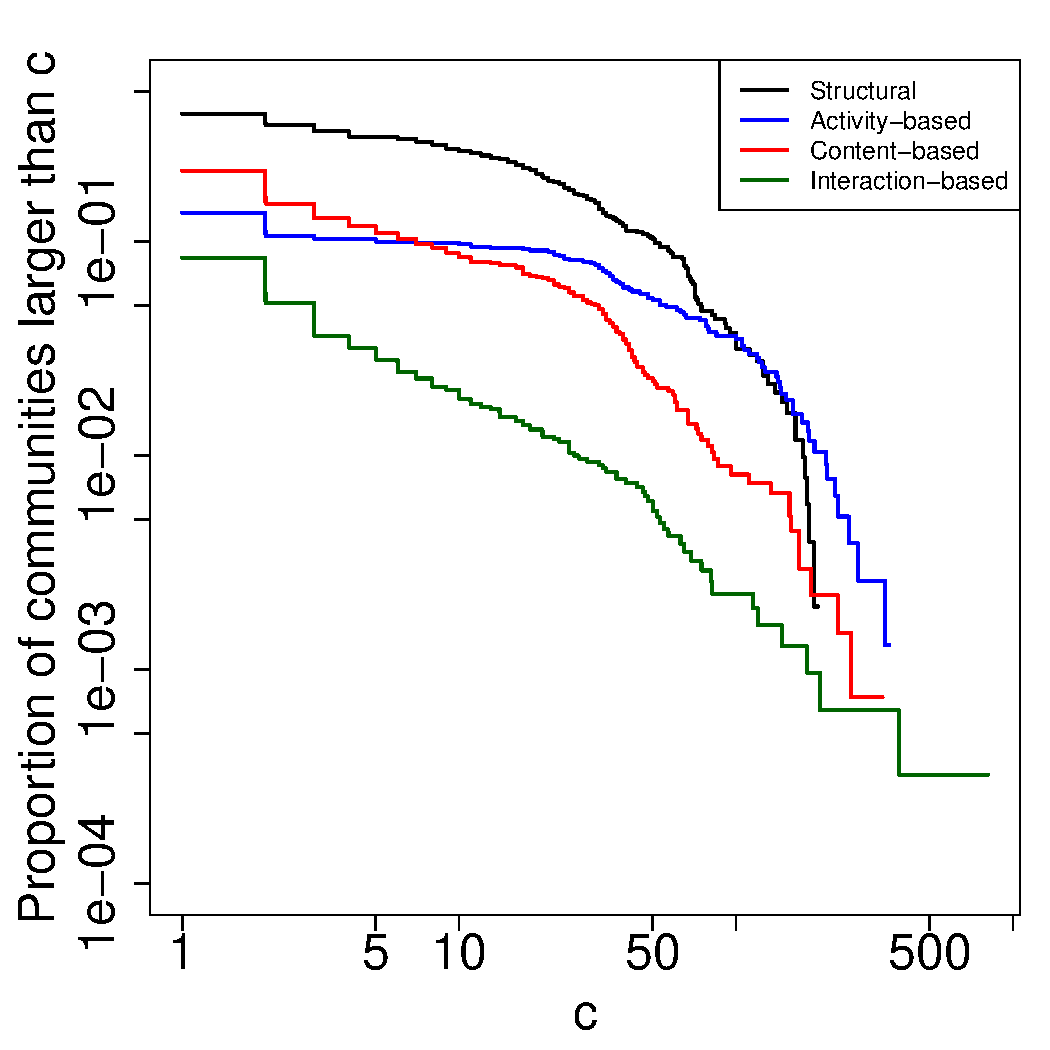
\includegraphics[width=0.50\textwidth]{comm_sizes_ecdf_loglog.pdf}
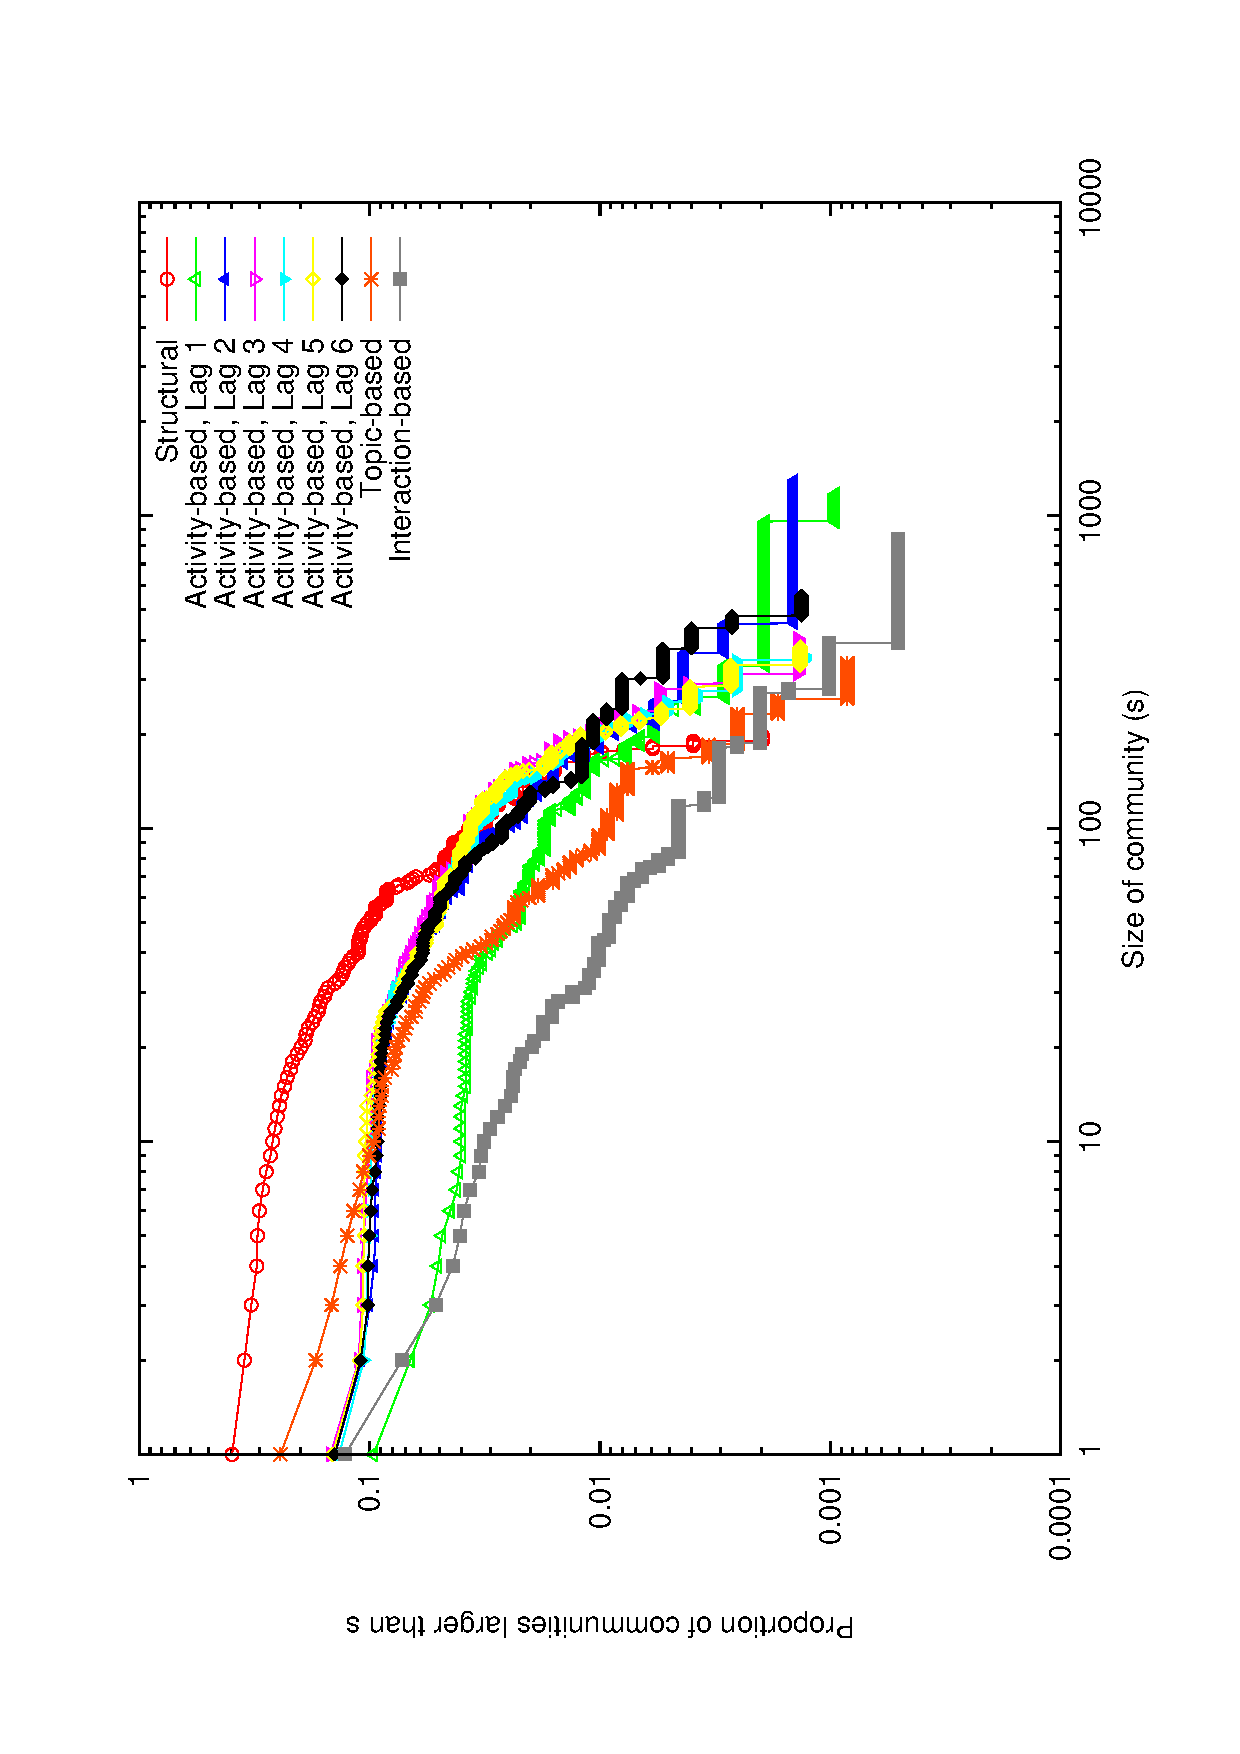
\includegraphics[width=1\textwidth]{cdf_comm_sizes}
\caption{The proportion of communities greater than $s$ in size, across the different community types. Note the logarithmic scale on the horizontal and vertical axes.}
\label{Fig-community_size_distribution}
\end{figure}

% Next, we compare the number of users which belong to more than one community. Figure~\ref{Fig-overlap_plot} shows the number of users belonging to 2, 3, or 4 communities. We see that as the number of mixed membership communities increases, the number of users with that number of mixed memberships decreases. This is especially true for the activity-based community \textbf{TK: speculate on what this means? Or save for the results section?}.  In addition, \textbf{TK: mention the 5, 6, and 7 cases, not included in the figure}. This corresponded to \textbf{TK: investigate which users are the high-overlap and what communities they belong to.}

% % The user with a structural overlap of 7 communities was 1630261,
% %	https://twitter.com/marksilva

% \begin{figure}[ht]
%   \centering
% 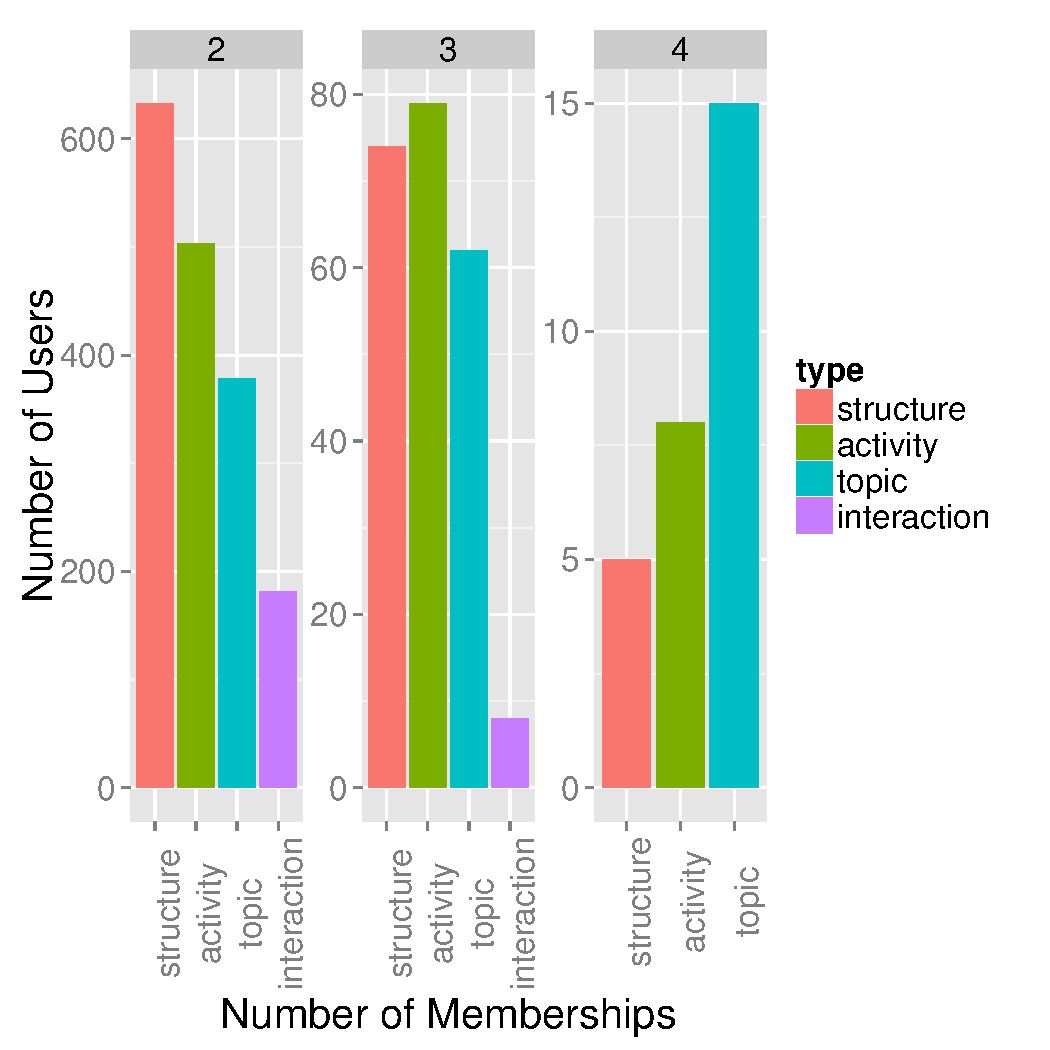
\includegraphics[width=0.50\textwidth]{Figures/overlap_by_type.pdf}
% \caption{The number of users belonging to 2, 3, or 4 communities, by community type.}
% \label{Fig-overlap_plot}
% \end{figure}

\subsection{Comparing Community Structure with Normalized Mutual Information}

In the previous section, we saw that the large scale statistics of the communities were highly dependent on the type of community under consideration. However, macroscale network statistics do not account for differences in community structure that result from operations such as splitting or merging of communities. Moreover, this view does not account for which users belong to which communities, and in particular which users belong to the same communities across community types. To answer this question, we invoke methods for the comparison of clusters: given two different clusterings of nodes into communities, how similar are the two clusters? The standard approach to answering this question is to define a metric on the space of possible partitions.  
Because we detect coverings rather than partitions, standard cluster comparison metrics like variation of information~\cite{meilua2003comparing} are not appropriate. Instead, we use a generalization of variation of information first introduced in~\cite{Lancichinetti2009}, the normalized mutual information. The normalized mutual information stems from treating clustering as a community identification problem: given that we know a node's community membership(s) in the first covering, how much information do we have about its community membership(s) in the second covering, and vice versa? Consider the two coverings $\mathcal{C}_{1}$ and $\mathcal{C}_{2}.$ We think of the community memberships of a randomly chosen node in $\mathcal{C}_{1}$ as a binary random vector $\mathbf{X} \in \{0, 1\}^{|\mathcal{C}_{1}|}$ where the $i^{\text{th}}$ entry of the vector is 1 if the node belongs to community $i$ and 0 otherwise. Similarly, $\mathbf{Y} \in \{ 0, 1\}^{|\mathcal{C}_{2}|}$ is a binary random vector indicating the community memberships of the node in $\mathcal{C}_{2}$. Then the normalized mutual information is defined as
\begin{align}
	\text{NMI}(\mathcal{C}_{1}, \mathcal{C}_{2}) = 1 - \frac{1}{2} \left( \frac{H[\mathbf{X} | \mathbf{Y}]}{H[\mathbf{X}]} + \frac{H[\mathbf{Y} | \mathbf{X}]}{H[\mathbf{Y}]}\right)
\end{align}
where $H[\cdot]$ denotes a marginal entropy and $H[\cdot | \cdot]$ denotes a conditional entropy. The normalized mutual information varies from 0 to 1, attaining the value of 1 only when $\mathcal{C}_{1}$ and $\mathcal{C}_{2}$ are identical coverings up to a permutation of their labels. See the appendix of~\cite{Lancichinetti2009} for more details.

We considered the normalized mutual information between the communities inferred from the structural network and the networks weighted with lag 1 through 6 transfer entropies, hashtag similarity, and mention, retweet, and mention-retweet activity. The resulting $\text{NMI}(\mathcal{C}_{i}, \mathcal{C}_{j})$ are shown in Figure~\ref{Fig-compare_coverings}. Note the block diagonal structure in Figure~\ref{Fig-compare_coverings}, which indicates that coverings are most similar within a question category. For example, the activity-based transfer entropy coverings are more similar to each other than to any of the other coverings. Similarly for the interaction-based mention, retweet, and mention-retweet coverings. This point may seem obvious, but the fact that the different weightings within a question category result in similar community structure indicates that each covering is capturing true, latent properties of the social network. Interestingly, the coverings resulting from the different weightings are all more similar to each other than to the structural covering from the unweighted network. Also note that the covering based on the hashtag similarities are different from all of the other weight-based coverings. In agreement with the results reported in the previous section, we see that the activity-based communities share similar structure for lags greater than 2. Because of these two results, in the remainder of the paper, we focus on the activity-based communities inferred using the lag-4 transfer entropy.

\begin{figure}[ht!]
  \centering
  \begin{tabu}{cl}
    \toprule
    Normalized Mutual Information & Community Types \\
    \midrule
    \multirow{8}[8]{*}{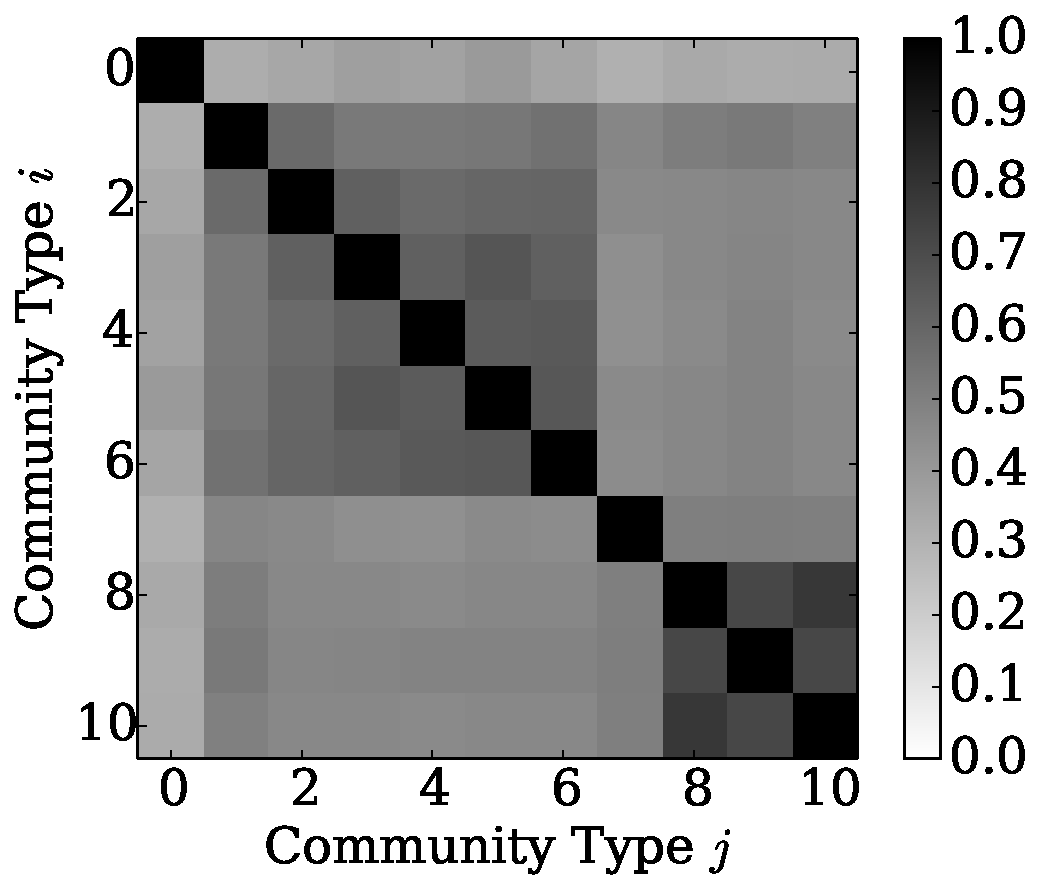
\includegraphics[width=0.50\textwidth]{nmi_singletons}}&0---Structural \bigstrut\\
    &1-6---Activity-Based with Lags 1-6\bigstrut\\
    %&2---Activity-Based with Lag 2\bigstrut\\
    %&3---Activity-Based with Lag 3\bigstrut\\
    %&4---Activity-Based with Lag 4\bigstrut\\
    %&5---Activity-Based with Lag 5\bigstrut\\
    %&6---Activity-Based with Lag 6\bigstrut\\
    &7---Topic-Based \bigstrut\\
    &8---Interaction-Based with Mentions\bigstrut\\
    &9---Interaction-Based with Retweets\bigstrut\\
    &10---Interaction-Based with both \bigstrut\\
    &\,\,\,\,\,\,\,\,\,\,\,\,\,\,Mentions and Retweets\bigstrut\\
    &\bigstrut\\
    \bottomrule
\end{tabu}
\caption{The normalized mutual information between the coverings inferred from the different community types. 
%Community type 0 corresponds to the structural communities, community types 1 through 6 correspond to the activity-based communities with lag 1 through 6 transfer entropies, community type 7 corresponds to the topic-based communities, and community types 8, 9, and 10 correspond to the interaction-based communities using mentions, retweets, and both mentions and retweets. 
Values of normalized mutual information close to 1 indicate similarity in the community structure, while values close to 0 indicate dissimilarity. The normalized mutual information is computed with singletons and orphan nodes included. Note the block-diagonal structure, indicating the strong relationship between question type and community membership.}
\label{Fig-compare_coverings}
\end{figure}

Thus, we see that although the activity-based, interaction-based, and topic-based communities relied on the structural network, their community structure differs \emph{the most} from the community structure of the follower network. This agrees with the results from the previous section, and reinforces that the follower network is a necessary but not sufficient part of detecting communities characterized by properties beyond follower-followee relationships.

%%%%%%%%%%%%%%%%%%%%%%%%%%%%%%%%%%%%%%%%%%%%%%%%%%%%%%%%%%%%% 
%============================================================
% Old section on 'Comparing Edges Across Different Community Types'

% \subsection{Comparing Edges Across Different Community Types}

% We next explore how the edge weights defined by equations (\ref{Eqn-EW-activity}), (\ref{Eqn-EW-interaction}), and (\ref{Eqn-EW-topic}), and thus different forms of information flow, differ between community types. For a fixed community type, edges for a particular community may be partitioned into three sets: those from a user in the community to another user in the community (internal-to-internal), those from a user in the community to a user outside of the community (internal-to-external), and those from a user outside the community to a user inside the community (external-to-internal). See Figure~\ref{Fig-edge_types} for a schematic of this edge partitioning. For a meaningful community, we expect the distribution of weights within the community (internal-to-internal weights) to be different from the distribution of weights without the community (internal-to-external and external-to-internal).

% \begin{figure}[ht]
%   \centering
% 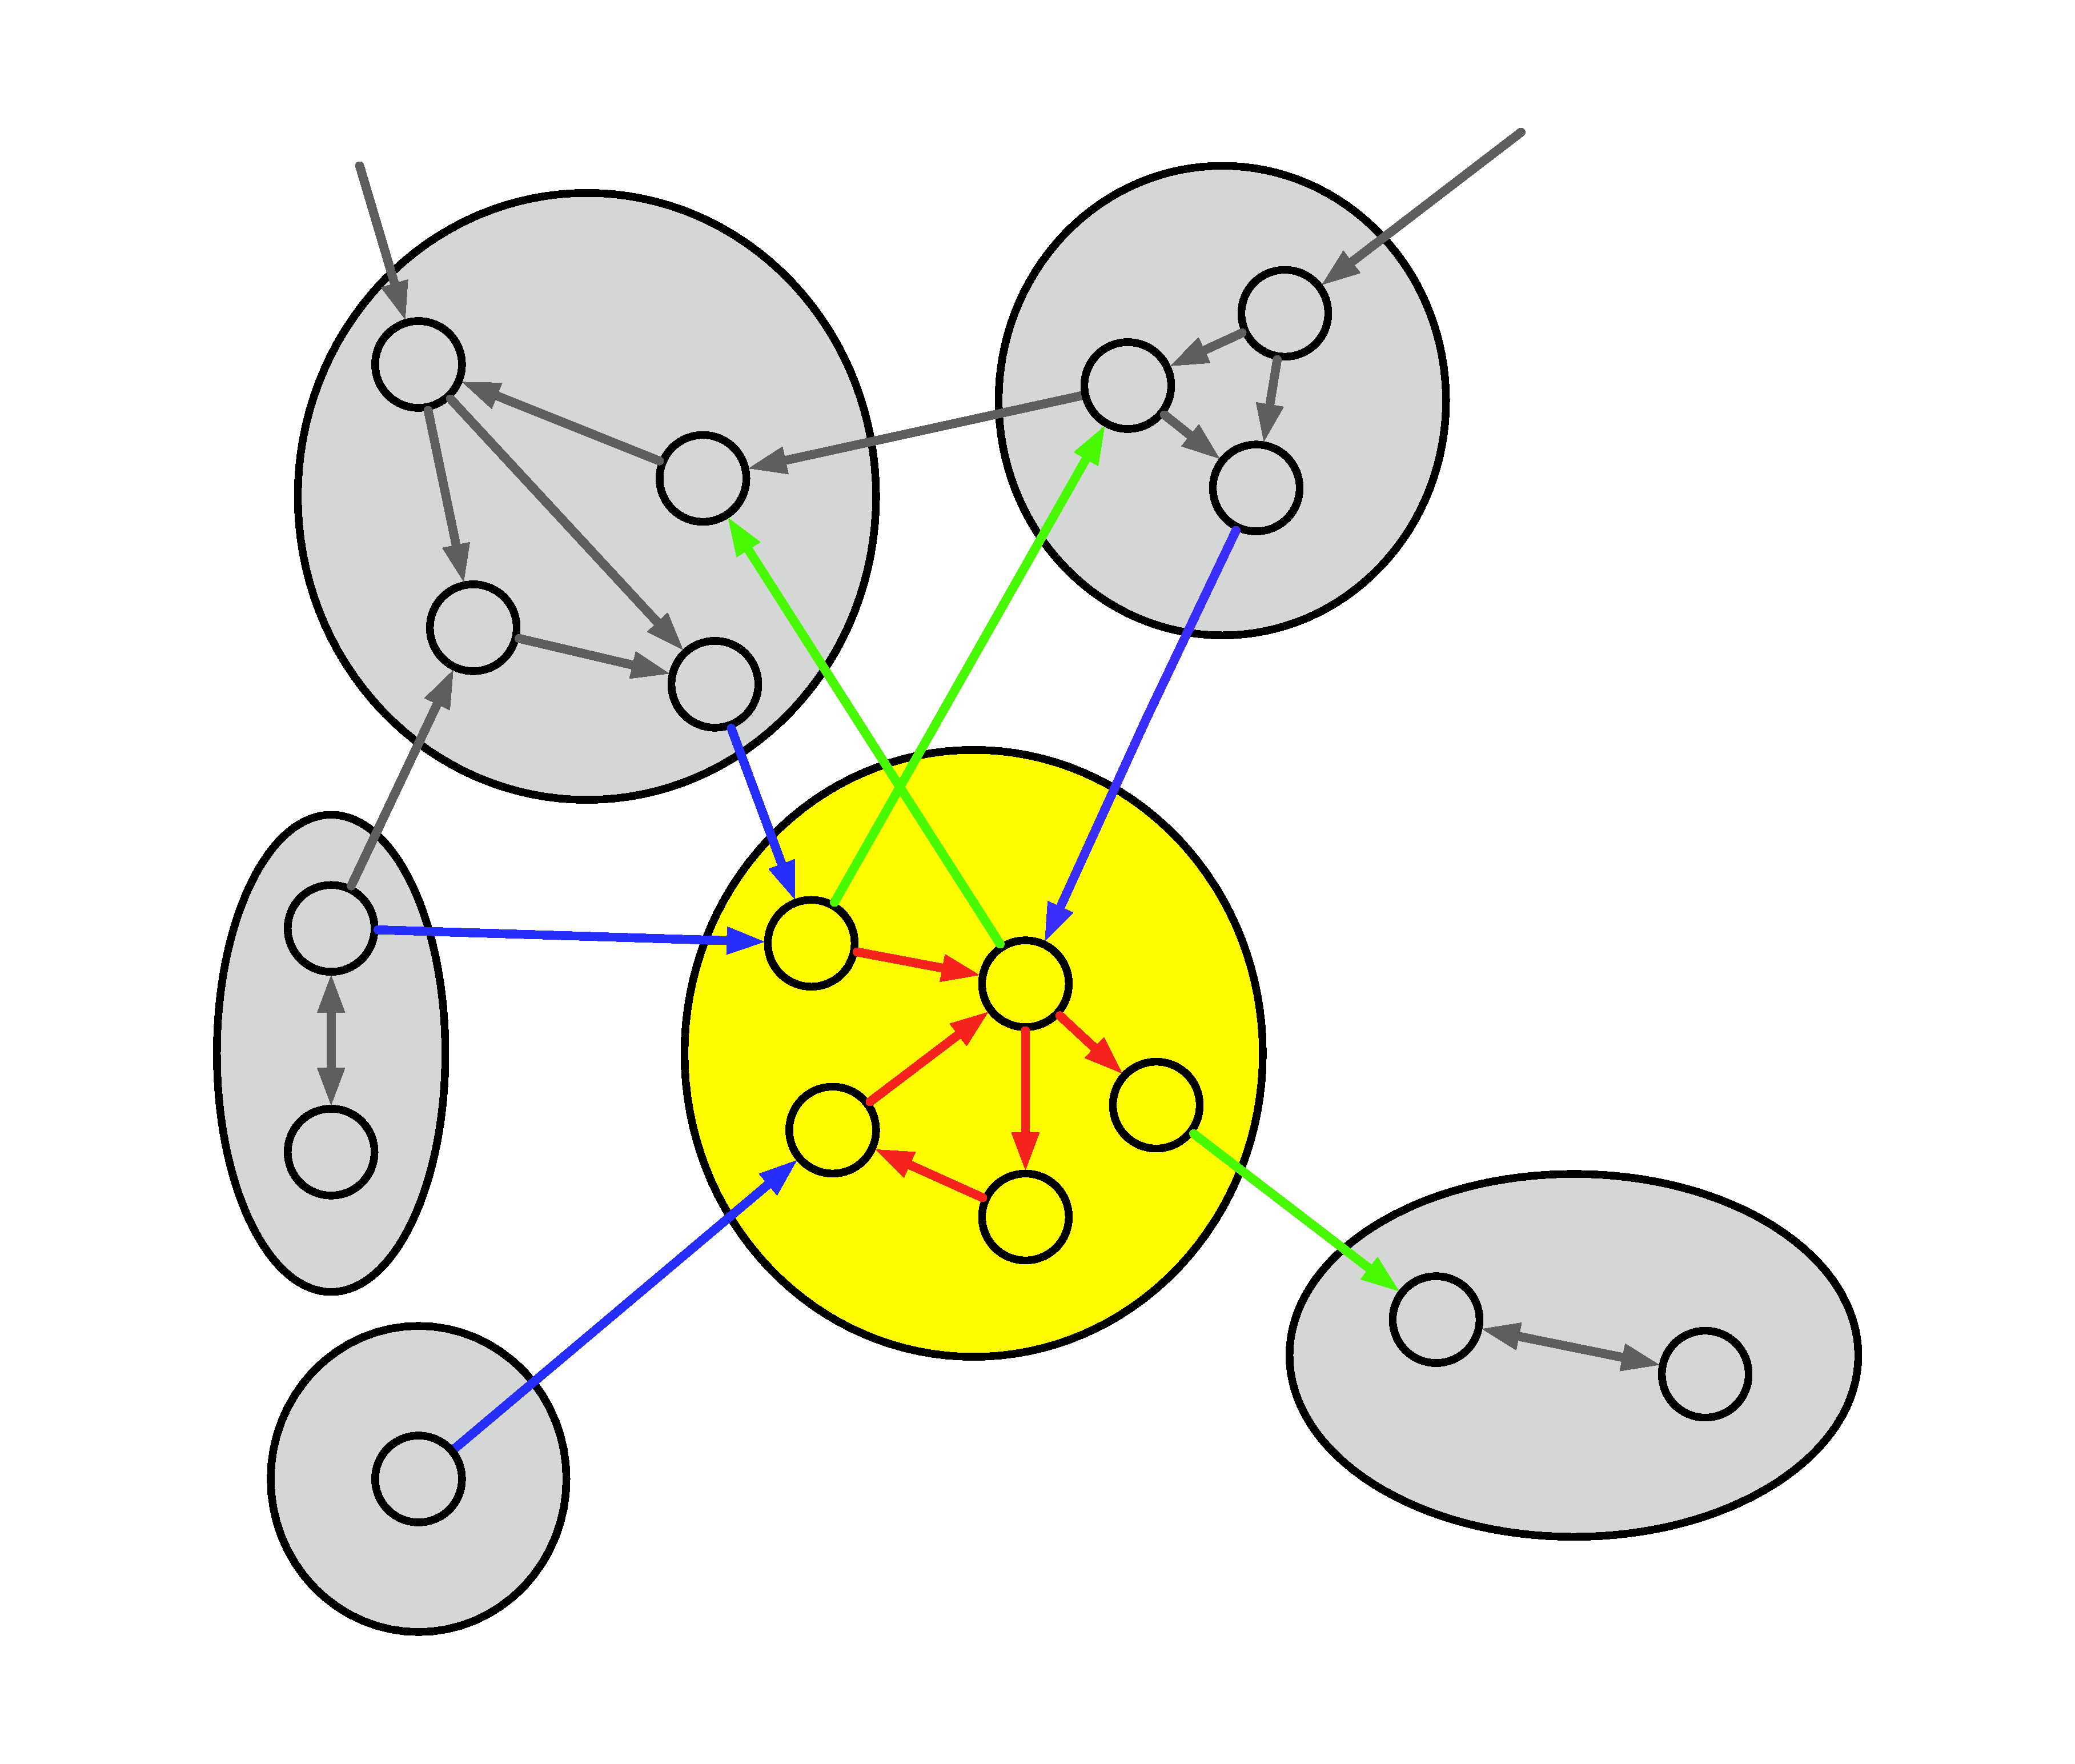
\includegraphics[width=0.50\textwidth]{edge-types.eps}
% \caption{An example of the edges considered in determining the edge weight distribution for a given community (the focal community is in yellow). We focus on the internal-to-internal (red), internal-to-external (green), and external-to-internal (blue) edges. For a given focal community, all other edges (grey) are not considered.}
% \label{Fig-edge_types}
% \end{figure}

% As an example, Figure~\ref{Fig-dist_across_community} shows the distributions of hashtag-based weights for the largest community in the mention-retweet network. We see that the distribution of internal-to-internal hashtag weights has a longer tail than either the external-to-internal or internal-to-external hashtag weights, with edges within the community having higher weights than edges crossing the boundary of the community. Thus, while the community was defined in terms of interactions, we still see a shift in the distribution of topic-similarity.

% \begin{figure}[ht]
%   \centering
% 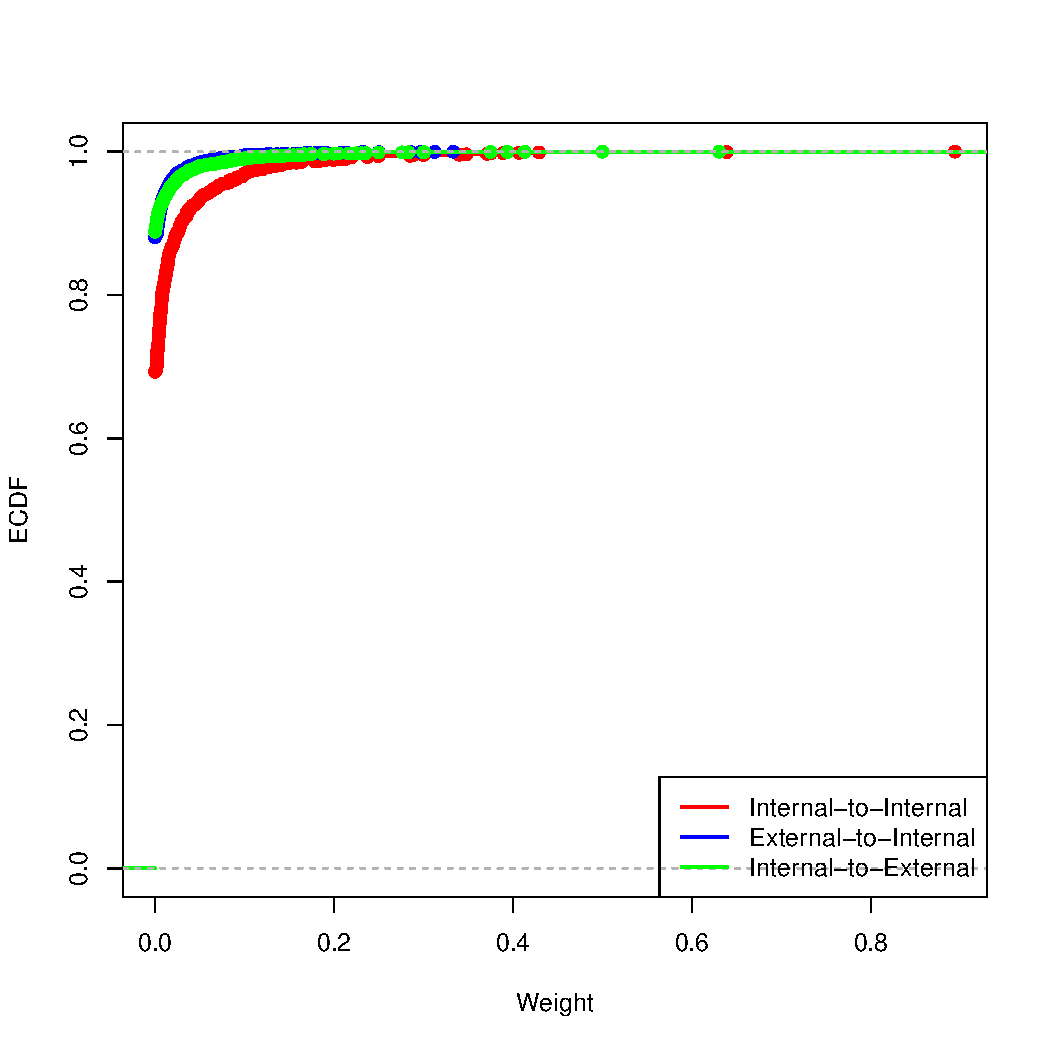
\includegraphics[width=0.50\textwidth]{comm0_labels-hashtag_weights-mention-retweet-ecdf.pdf}
% \caption{The proportion of edges with a weight at least as large as the weight on the horizontal axis, across the types of edges described in Figure~\ref{Fig-edge_types}. The community is defined by user interactions, and the edge weights are determined by topic similarity. The dashed vertical lines indicate the median weight for each type of edge. Note the logarithmic scale on the horizontal axis.}
% \label{Fig-dist_across_community}
% \end{figure}

% \begin{figure}
%         \centering
%         \begin{subfigure}[b]{0.2\textwidth}
%                 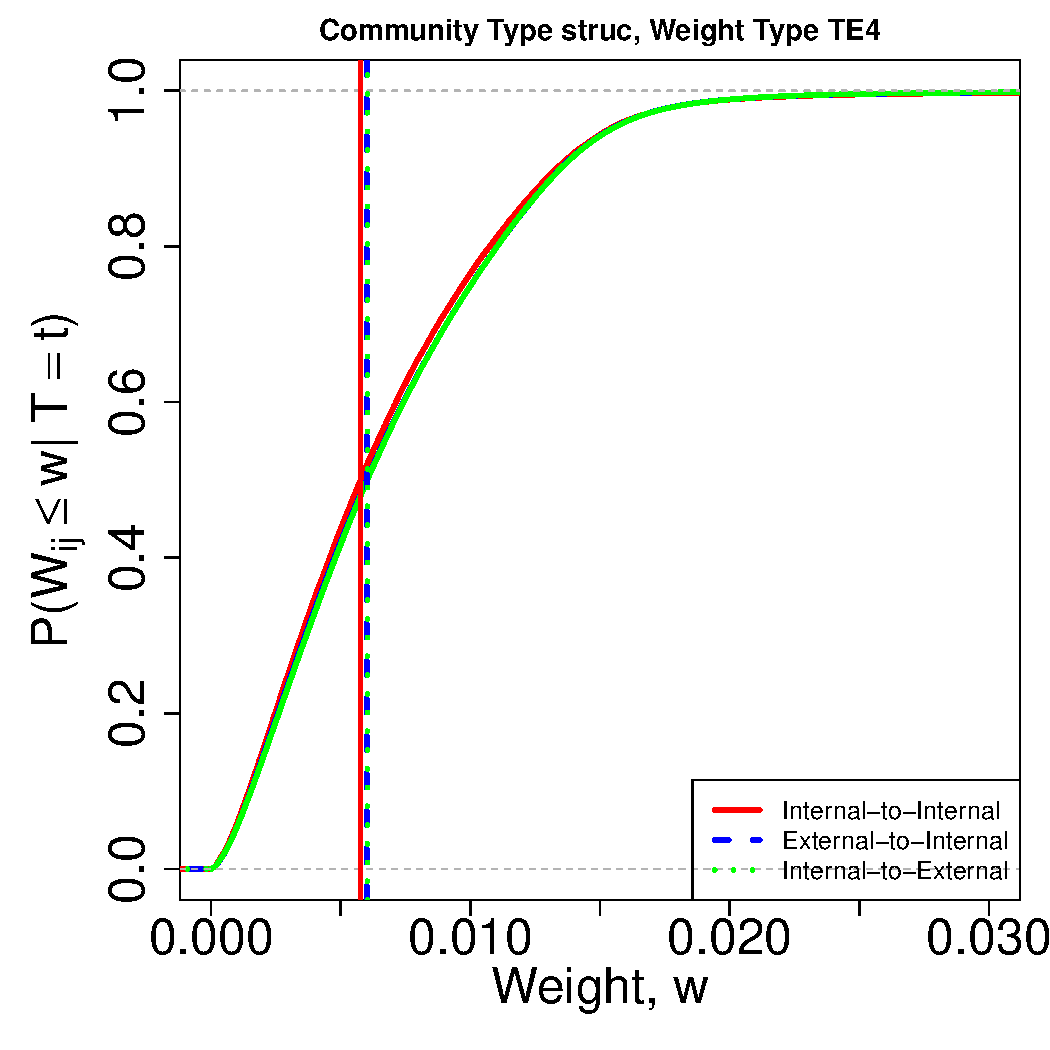
\includegraphics[width=\textwidth]{labels-struc_weights-TE4-ecdf_by_type.pdf}
%         \end{subfigure}
%         \begin{subfigure}[b]{0.2\textwidth}
%                 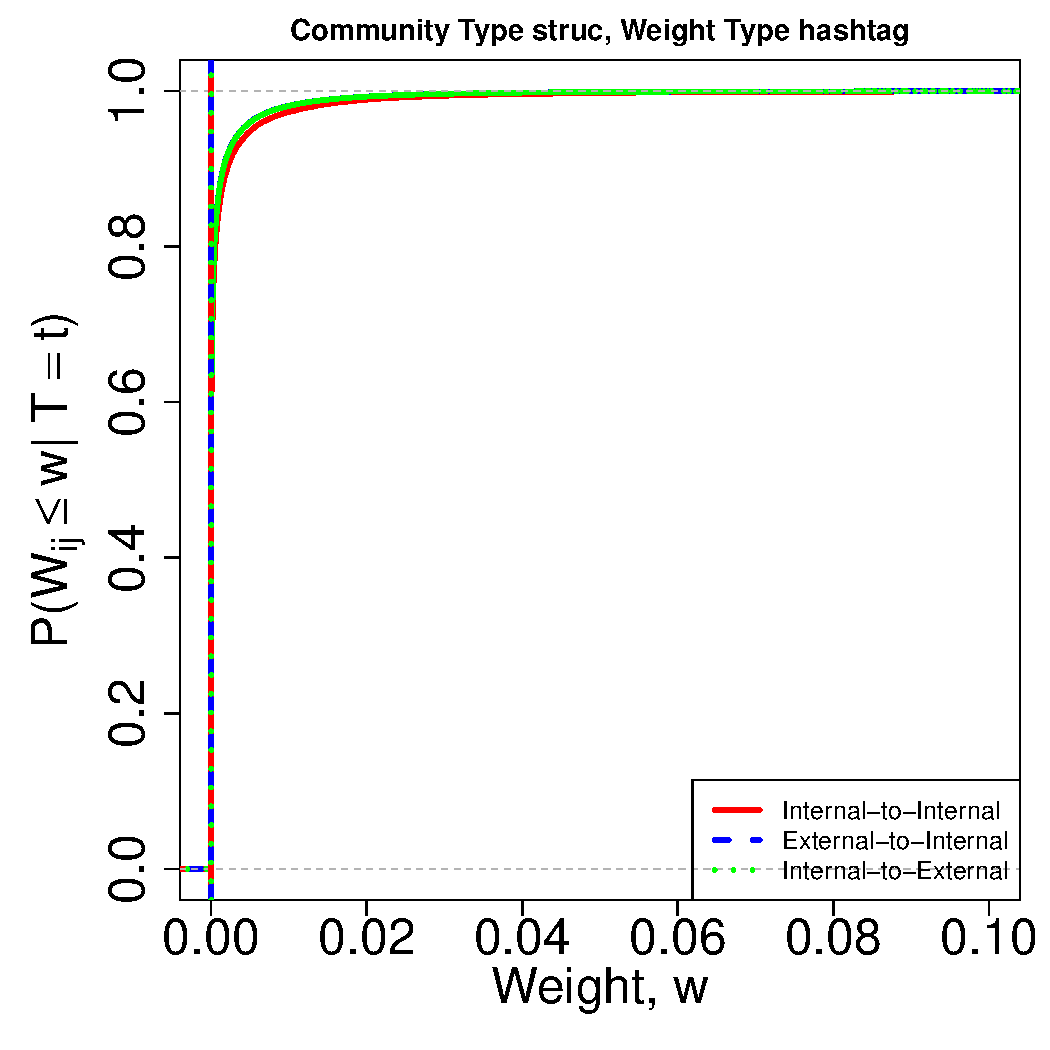
\includegraphics[width=\textwidth]{labels-struc_weights-hashtag-ecdf_by_type.pdf}
%         \end{subfigure}
%         \begin{subfigure}[b]{0.2\textwidth}
%                 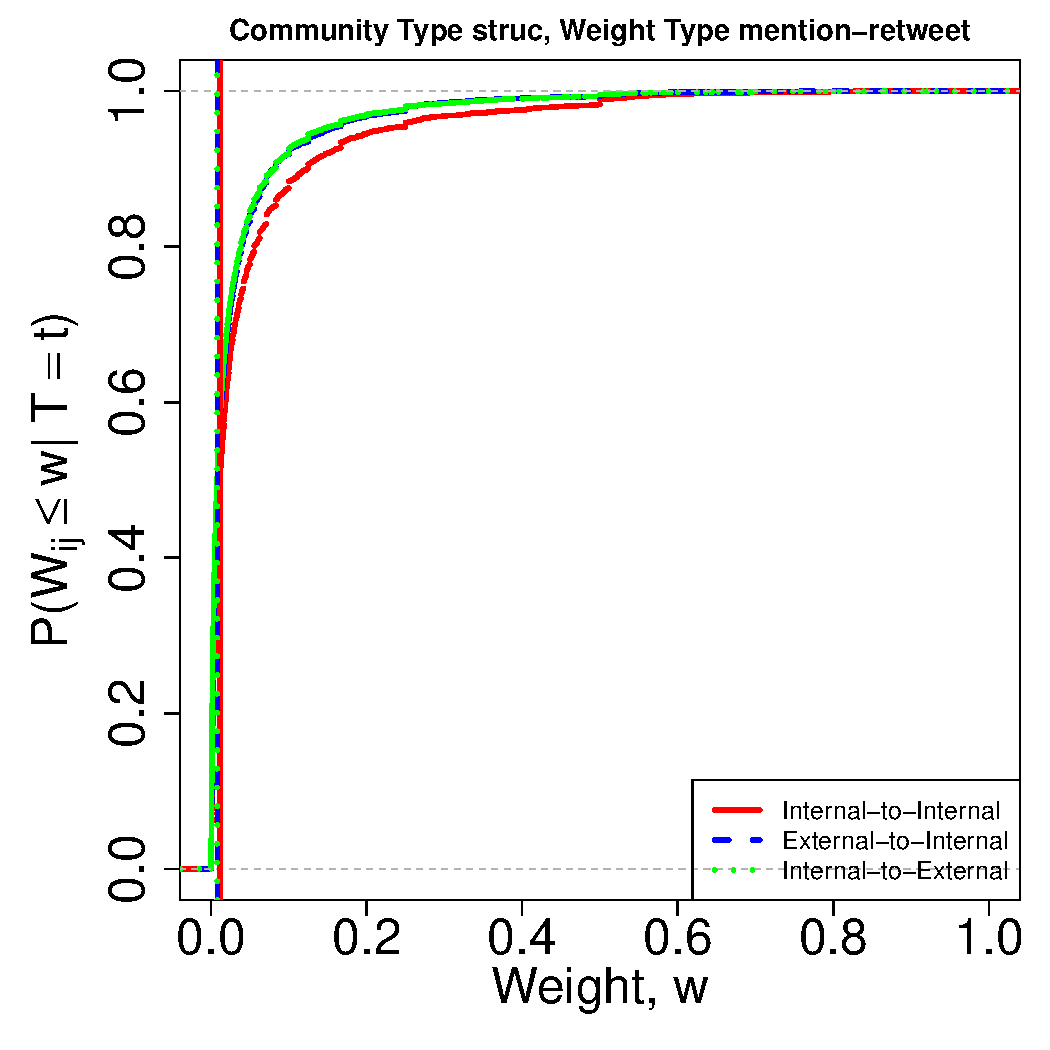
\includegraphics[width=\textwidth]{labels-struc_weights-mention-retweet-ecdf_by_type.pdf}
%         \end{subfigure}
%         \caption{Lorem ipsum.}
% \end{figure}

% This change in the tail of the distribution between edge types was typical of many of the community type / weight pairings. A useful summary statistic to quantify the change involves the median weights across the three types of edges, as demonstrated in Figure~\ref{Fig-dist_across_community}. In particular, by computing the ratio of the median weight for the internal-to-internal edges to the median weight for the internal/external-to-external/internal edges, we can quantify the ratio change in weight strength internal vs. external to a community. We computed this quantity for each of the top 100 largest communities defined by a particular community type (structure-based, activity-based, interaction-based, or topic-based), and report the median value across the 100 largest communities for each type in Table~\ref{Table-medians}. This statistic represents the typical ratio shift for each community type / weight pairing. Values greater than 1 indicate that the edge weights tend to be higher within the community, and values less than 1 indicate that the edge weights tend to be higher for those edges crossing the community boundary.

% \begin{table}
% 	\caption{The median value for the ratio of the median external/internal-to-internal/external weight to median internal-to-internal weight for the different community/weight pairings.}
% 	\centering
% 	\begin{tabular}{c | c | c  c  c  c}
% 		& & \multicolumn{4}{ c }{Community} \\ \hline
% 		\multirow{4}{*}{Weight} & & S & TE & MR & HT \\ \hline
% 		& TE & $0.0 / 0.0$ & $0.0 / 0.0$ & $0.0 / 0.0$ & $0.0 / 0.0$\\
% 		& MR & $0.0 / 0.0$ & $0.0 / 0.0$ & $0.0 / 0.0$ & $0.0 / 0.0$\\
% 		& HT & $0.0 / 0.0$ & $0.0 / 0.0$ & $0.0 / 0.0$ & $0.0 / 0.0$
% 	\end{tabular}
% \end{table}

% \begin{table}
% 	\label{Table-medians}
% 	\caption{The median value across the 100 largest communities for the ratio of the median internal-to-internal weight to the median external-to-internal / internal-to-external weight for the different community / weight pairings. Note: For mention-retweet weights, weight zero edges were excluded from the computation of the median. We indicate such cases with an asterisk.}
% 	\centering
% 	\begin{tabular}{c | c | c  c  c}
% 		& & \multicolumn{3}{ c }{Weight Type} \\ \cline{3-5}
% 		& & TE & MR & HT \\ \cline{2-5}
% 		\multirow{4}{*}{Community Type} & S & $0.96/0.94$& $1.7/2.1$*& $9.0/8.0$\\
% 		& A & $1.0/0.96$& $1.5/2.4$*& $24/17$\\
% 		& I & $0.83/0.86$& $3.2/4.4$& $10/8.5$\\
% 		& T & $0.9/0.89$& $2.4/2.6$*& $28/26$
% 	\end{tabular}
% \end{table}

% \begin{table}
% 	\caption{The median value across the 100 largest communities for the ratio of the median internal-to-internal weight to the median external-to-internal / internal-to-external weight for the different community / weight pairings. For each entry $a/b$ in the table, $a$ corresponds to median ratio value for edges external-to-internal, and $b$ corresponds to the median ratio value for edges internal-to-external . Community types correspond to S(tructural), A(ctivity-based), T(opic-based), and I(nteraction-based) communities. Weight types correspond to T(ransfer) E(ntropy), M(ention-)R(etweet), and H(ash)T(ag). Note: For mention-retweet weights, zero weight edges were excluded from the computation of the median. We indicate such cases with an asterisk.}
% 	\centering
% 	\begin{tabular}{c  c | c  c  c}
% 		& & \multicolumn{3}{ c }{Weight Type} \\ %\cline{3-5}
% 		& & TE & MR & HT \\ \cline{1-5}
% 		\multirow{4}{*}{Community} & S & $0.96/0.94$& $1.7/2.1$*& $9.0/8.0$\\
% 		\multirow{4}{*}{Type} & A & $1.0/0.96$& $1.5/2.4$*& $24/17$\\
% 		& I & $0.83/0.86$& $3.2/4.4$& $10/8.5$\\
% 		& T & $0.9/0.89$& $2.4/2.6$*& $28/26$
% 	\end{tabular}
% 	\label{Table-medians}
% \end{table}

% We see that for every weight type except transfer entropy, the weight on edges internal to the communities tend to be higher than on edges entering or exiting the communities, ranging from a factor of 1.5 times larger for the activity-based/mention-retweet pairing to a factor of 28 times larger for the topic-based/hashtag similarity pairing. As stated above, we expect this ratio to be high for community / weight pairings that match (e.g. considering mention-retweet weighting for interaction-based communities), and we see that this is the case for all but the activity-based / transfer entropy pairing. Moreover, for both the mention-retweet and hashtag weightings, the ratio is largest when they match with the interaction-based and topic-based communities, respectively.

% For all four community types, the transfer entropy tended to be higher for edges crossing community boundaries than for those internal to community boundaries. Recall that the transfer entropy $\text{TE}_{X(u) \to X(f)}$ quantifies the reduction in uncertainty about a follower $f$'s activity from knowing the activity of a user $u$. This result therefore implies that, in terms of prediction, it is more useful to know the time series of a user followed outside of the community compared to a user followed inside of the community. Thus, in an information theoretic sense, we see that novel information useful for prediction is more likely to flow \emph{across} community boundaries than \emph{within} community boundaries.

% Note that the communities defined by the follower network do tend to have higher edge weights internal compared to across community boundaries. Thus, we do see that the structural communities capture some information about the functional behavior of communities of users in terms of topics and interaction. However, the ratio is not as large as when we explicitly seek out communities based on a particular type of functional community. This again emphasizes the importance of properly formulating the goal of a community detection study in the context of online social networks.

% \begin{tabular}{cc|ccc}
% & & \multicolumn{3}{ c| }{Weight Type} \\ \cline{3-5}
% & & 2 & 3 & 5  \\ \cline{1-5}
% \multicolumn{1}{ c| }{\multirow{4}{*}{Powers} } &
% \multicolumn{1}{ c| }{504} & 3 & 2 & 0    \\ \cline{2-5}
% \multicolumn{1}{ c|  }{}                        &
% \multicolumn{1}{ c| }{540} & 2 & 3 & 1     \\
% \multicolumn{1}{ c| }{gcd} & 2 & 2 & 0 \\ \cline{2-5}
% \multicolumn{1}{ c  }{}                        &
% \multicolumn{1}{ c| }{lcm} & 3 & 3 & 1 \\ \cline{1-5}
% \end{tabular}

%%%%%%%%%%%%%%%%%%%%%%%%%%%%%%%%%%%%%%%%%%%%%%%%%%%%%%%%%%%%% 
%============================================================

%%%%%%%%%%%%%%%%%%%%%%%%%%%%%%%%%%%%%%%%%%%%%%%%%%%%%%%%%%%%% 
%============================================================
% New section on 'Comparing Edges Across Different Community Types'

\subsection{Comparing Edges Across Different Community Types}

Any covering determined by OSLOM induces a natural partition of the edges in a directed network. In particular, let $u$ and $f$ be two users in the network, and let $M_{u}$ and $M_{f}$ be their community memberships. Then any edge $e_{u \to f}$ can be partitioned into one of three classes by
\begin{align}
	T(e_{u \to f}) = \left\{ \begin{array}{ll}
		\text{Inter-edge} &: \ \ \ M_{u} \cap M_{f} = \emptyset \\
		\text{Intra-edge} &: \ \ \ M_{u} = M_{f}\\
		\text{Mixed-edge} &: \ \ \ \text{ otherwise} \\
	\end{array}\right. \label{Eqn-edge_types}.
\end{align}
In words, an inter-edge connects two users who share no community memberships, an intra-edge connects two users who each belong to the same communities, and a mixed-edge connects two users who share some, but not all, community memberships. Thus, inter-edges cross community boundaries, intra-edges lie within community boundaries, and mixed-edges lie at the borders of community boundaries. See Figure~\ref{Fig-edge_types} for a schematic of this edge partitioning.

\begin{figure}[!h]
	\centering
	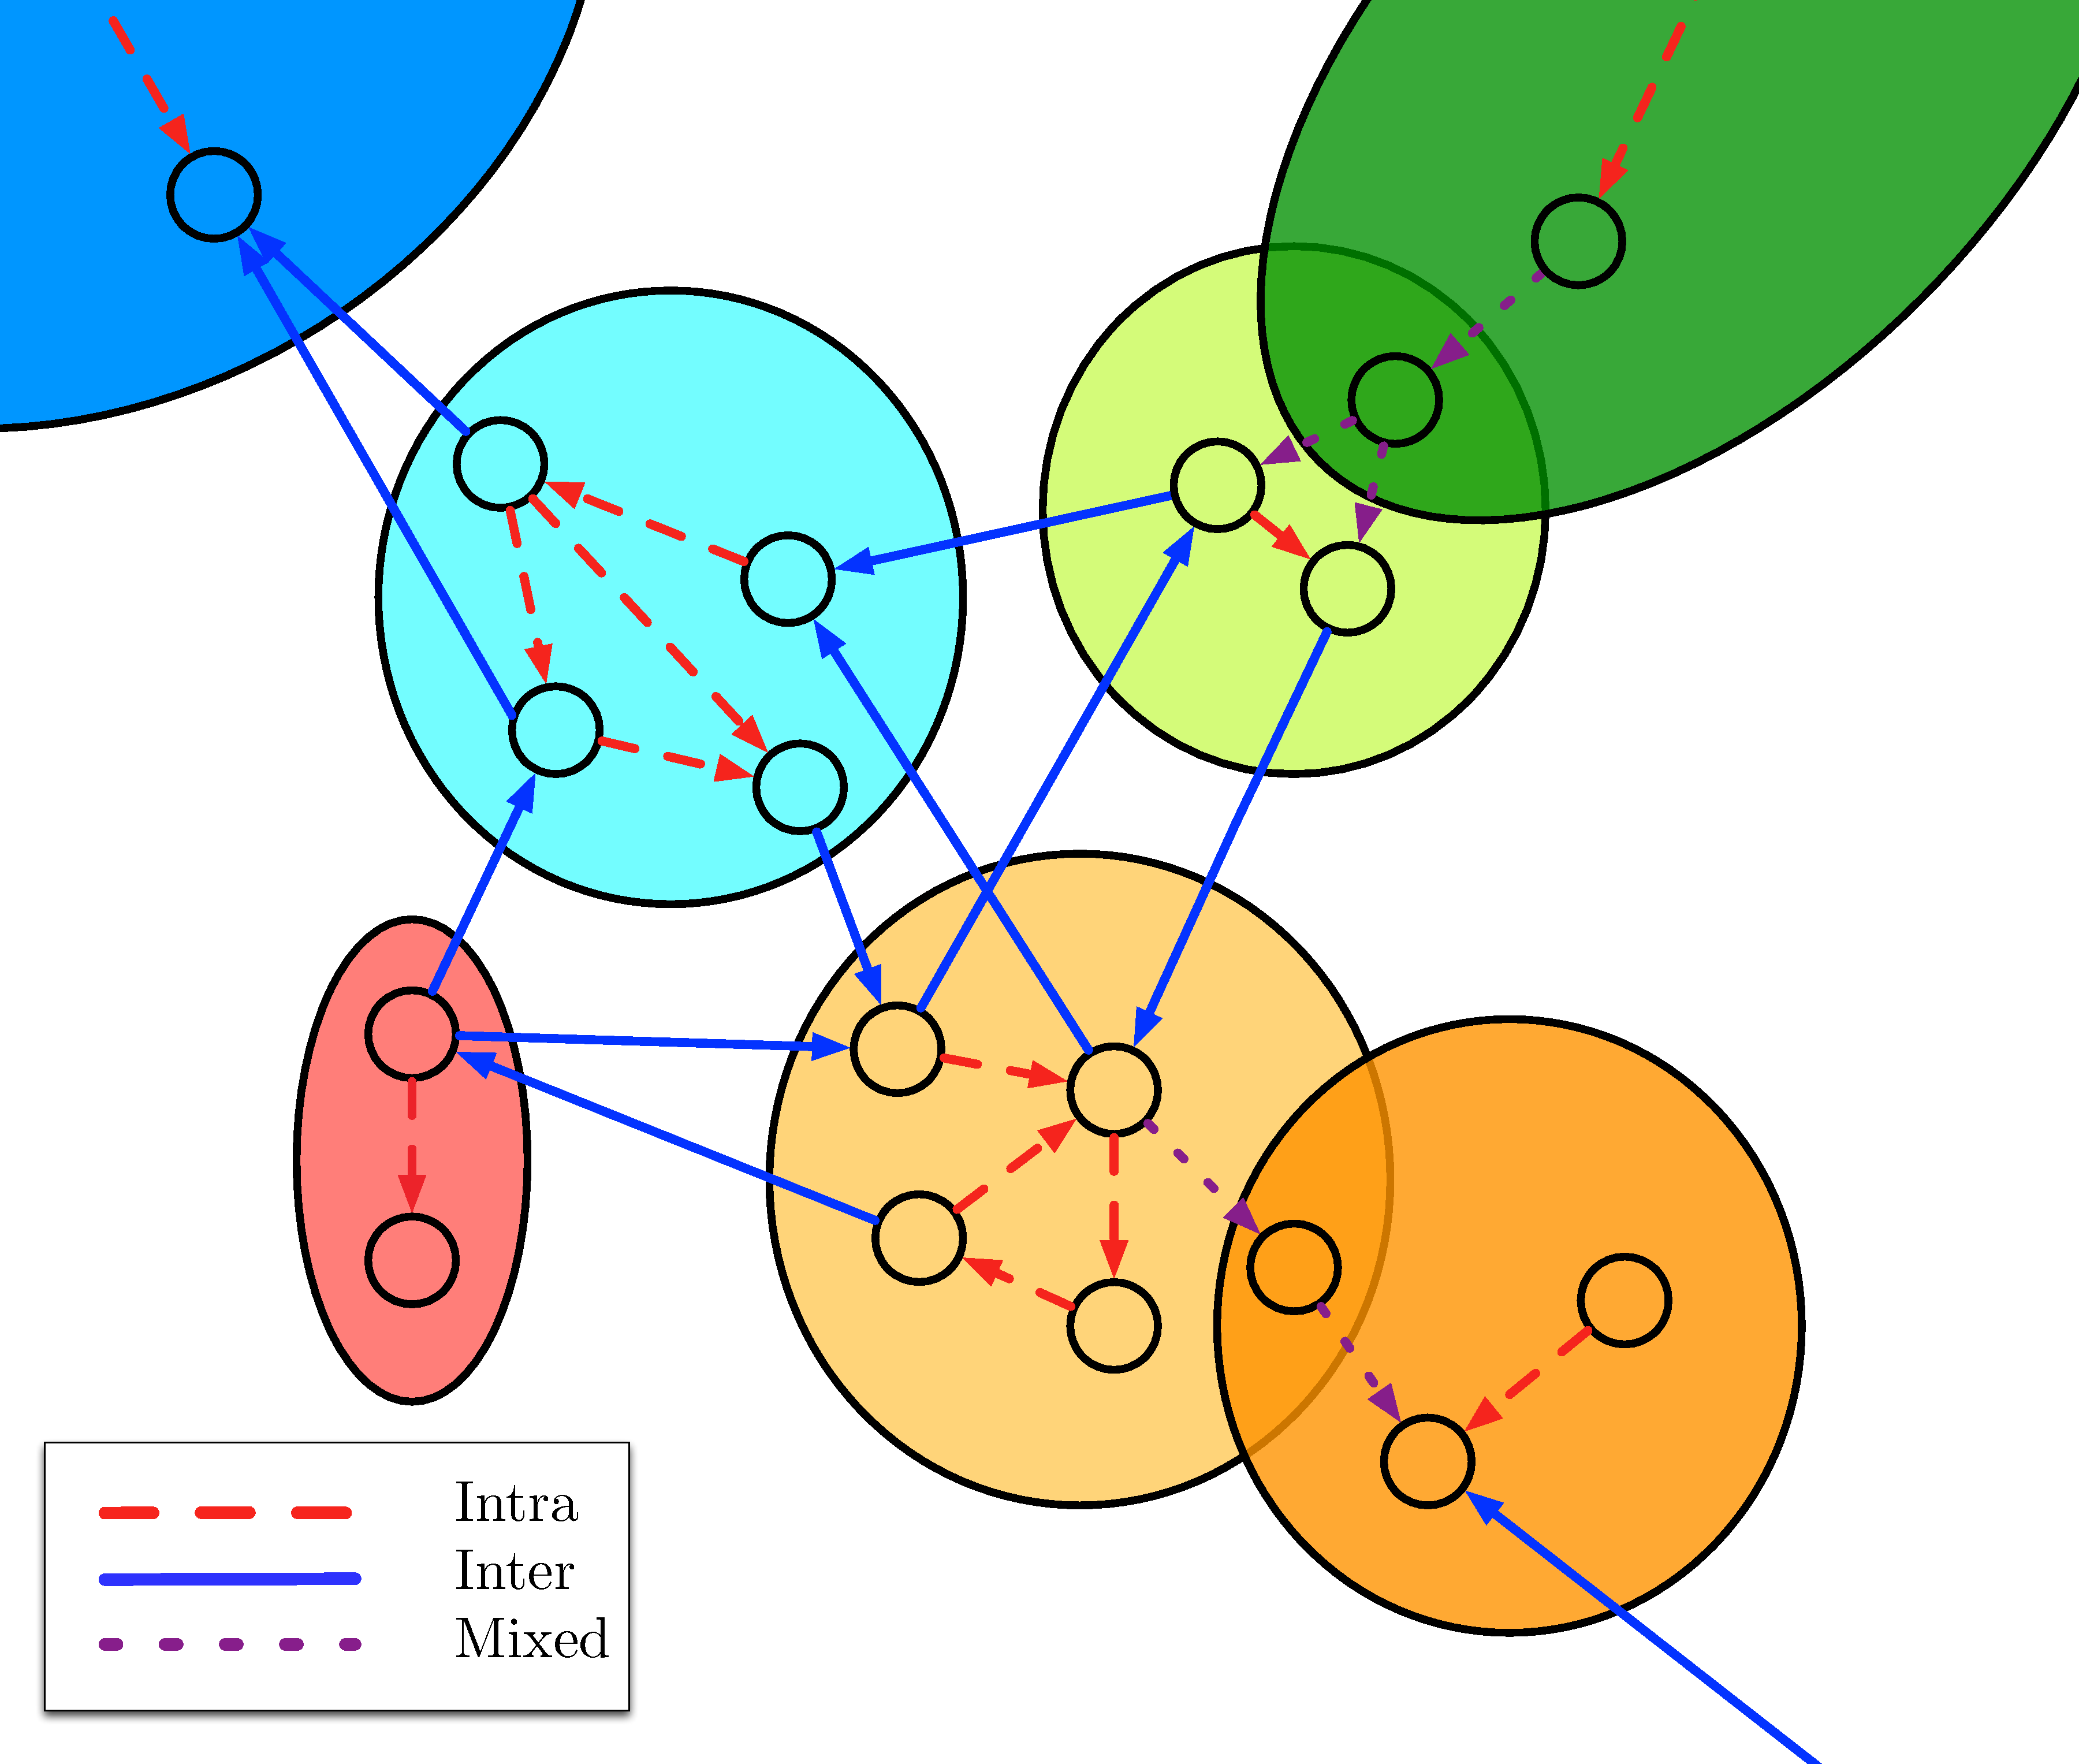
\includegraphics[width=0.8\textwidth]{edge-types}
	\caption{A schematic of how, given a covering, the edges of the network can be partitioned using (\ref{Eqn-edge_types}) into inter-edges, intra-edges, and mixed-edges. Inter-edges (red dashed) cross community boundaries. Intra-edges (blue solid) remain inside community boundaries. Mixed-edges (purple dotted) both remain in and cross community boundaries due to overlap in community membership. Each column corresponds to the same collection of weights, but partitioned using a different covering. Each row corresponds to the same covering, but for the different weights.}
	\label{Fig-edge_types}
\end{figure}

%\begin{table}
%	\caption{The percentage of intra-, inter-, and mixed-edges associated %with the coverings for each of the four community types.}
%	\centering
%	\begin{tabular}{l | r r r}
%		Community Type & Intra & Inter & Mixed \\
%		\hline
%		Structural & 7.5 & 87.0 &  5.5 \\
%		Activity-based & 10.7 & 81.9 & 7.4 \\
%		Topic-based & 7.3 & 89.0  & 3.7 \\
%		Interaction-based & 42.3 & 47.9 & 9.8
%	\end{tabular}
%\end{table}

Each community type (Structural, Activity-based, Topic-based, Interaction-based) induces a different partition of the edges, and each edge type (Transfer Entropy, Hashtag, Mention-Retweet) induces a different distribution of weights. That is, let $W_{u \to f}$ be the weight on an edge $E_{u \to f}$ chosen uniformly at random from the network, and compute
\begin{align}
	P(W_{u \to f} \leq w_{u \to f} | T(E_{u \to f}) = t),
\end{align}
the empirical distribution over the edge weights conditioned on the edge type $t$ being one of inter, intra, and mixed. The densities associated with these distributions are shown in Figure~\ref{Fig-distributions_by_types}. By considering how the weights vary conditional on the edge type, we can explore whether and how each of the follower-, interaction-, activity-, and topic-based communities define functional units within the network. For example, if users interact more-or-less independently of the topics they discuss, then the distributions of the interaction-based / topic-based edge weights should be independent of the edge type determined from the topic-based / interaction-based communities. By contrast, if users tend to interact mostly with those users who discuss similar topics, then the edge weight distributions should vary with the edge type.
%For meaningful community structure, we expect the distribution of edge weights to differ with the edge type $t$. If the community structure were arbitrary, the edge weights would be independent of the edge type, and all three conditional distributions would be identical.
\begin{figure}[!h]
	\centering
	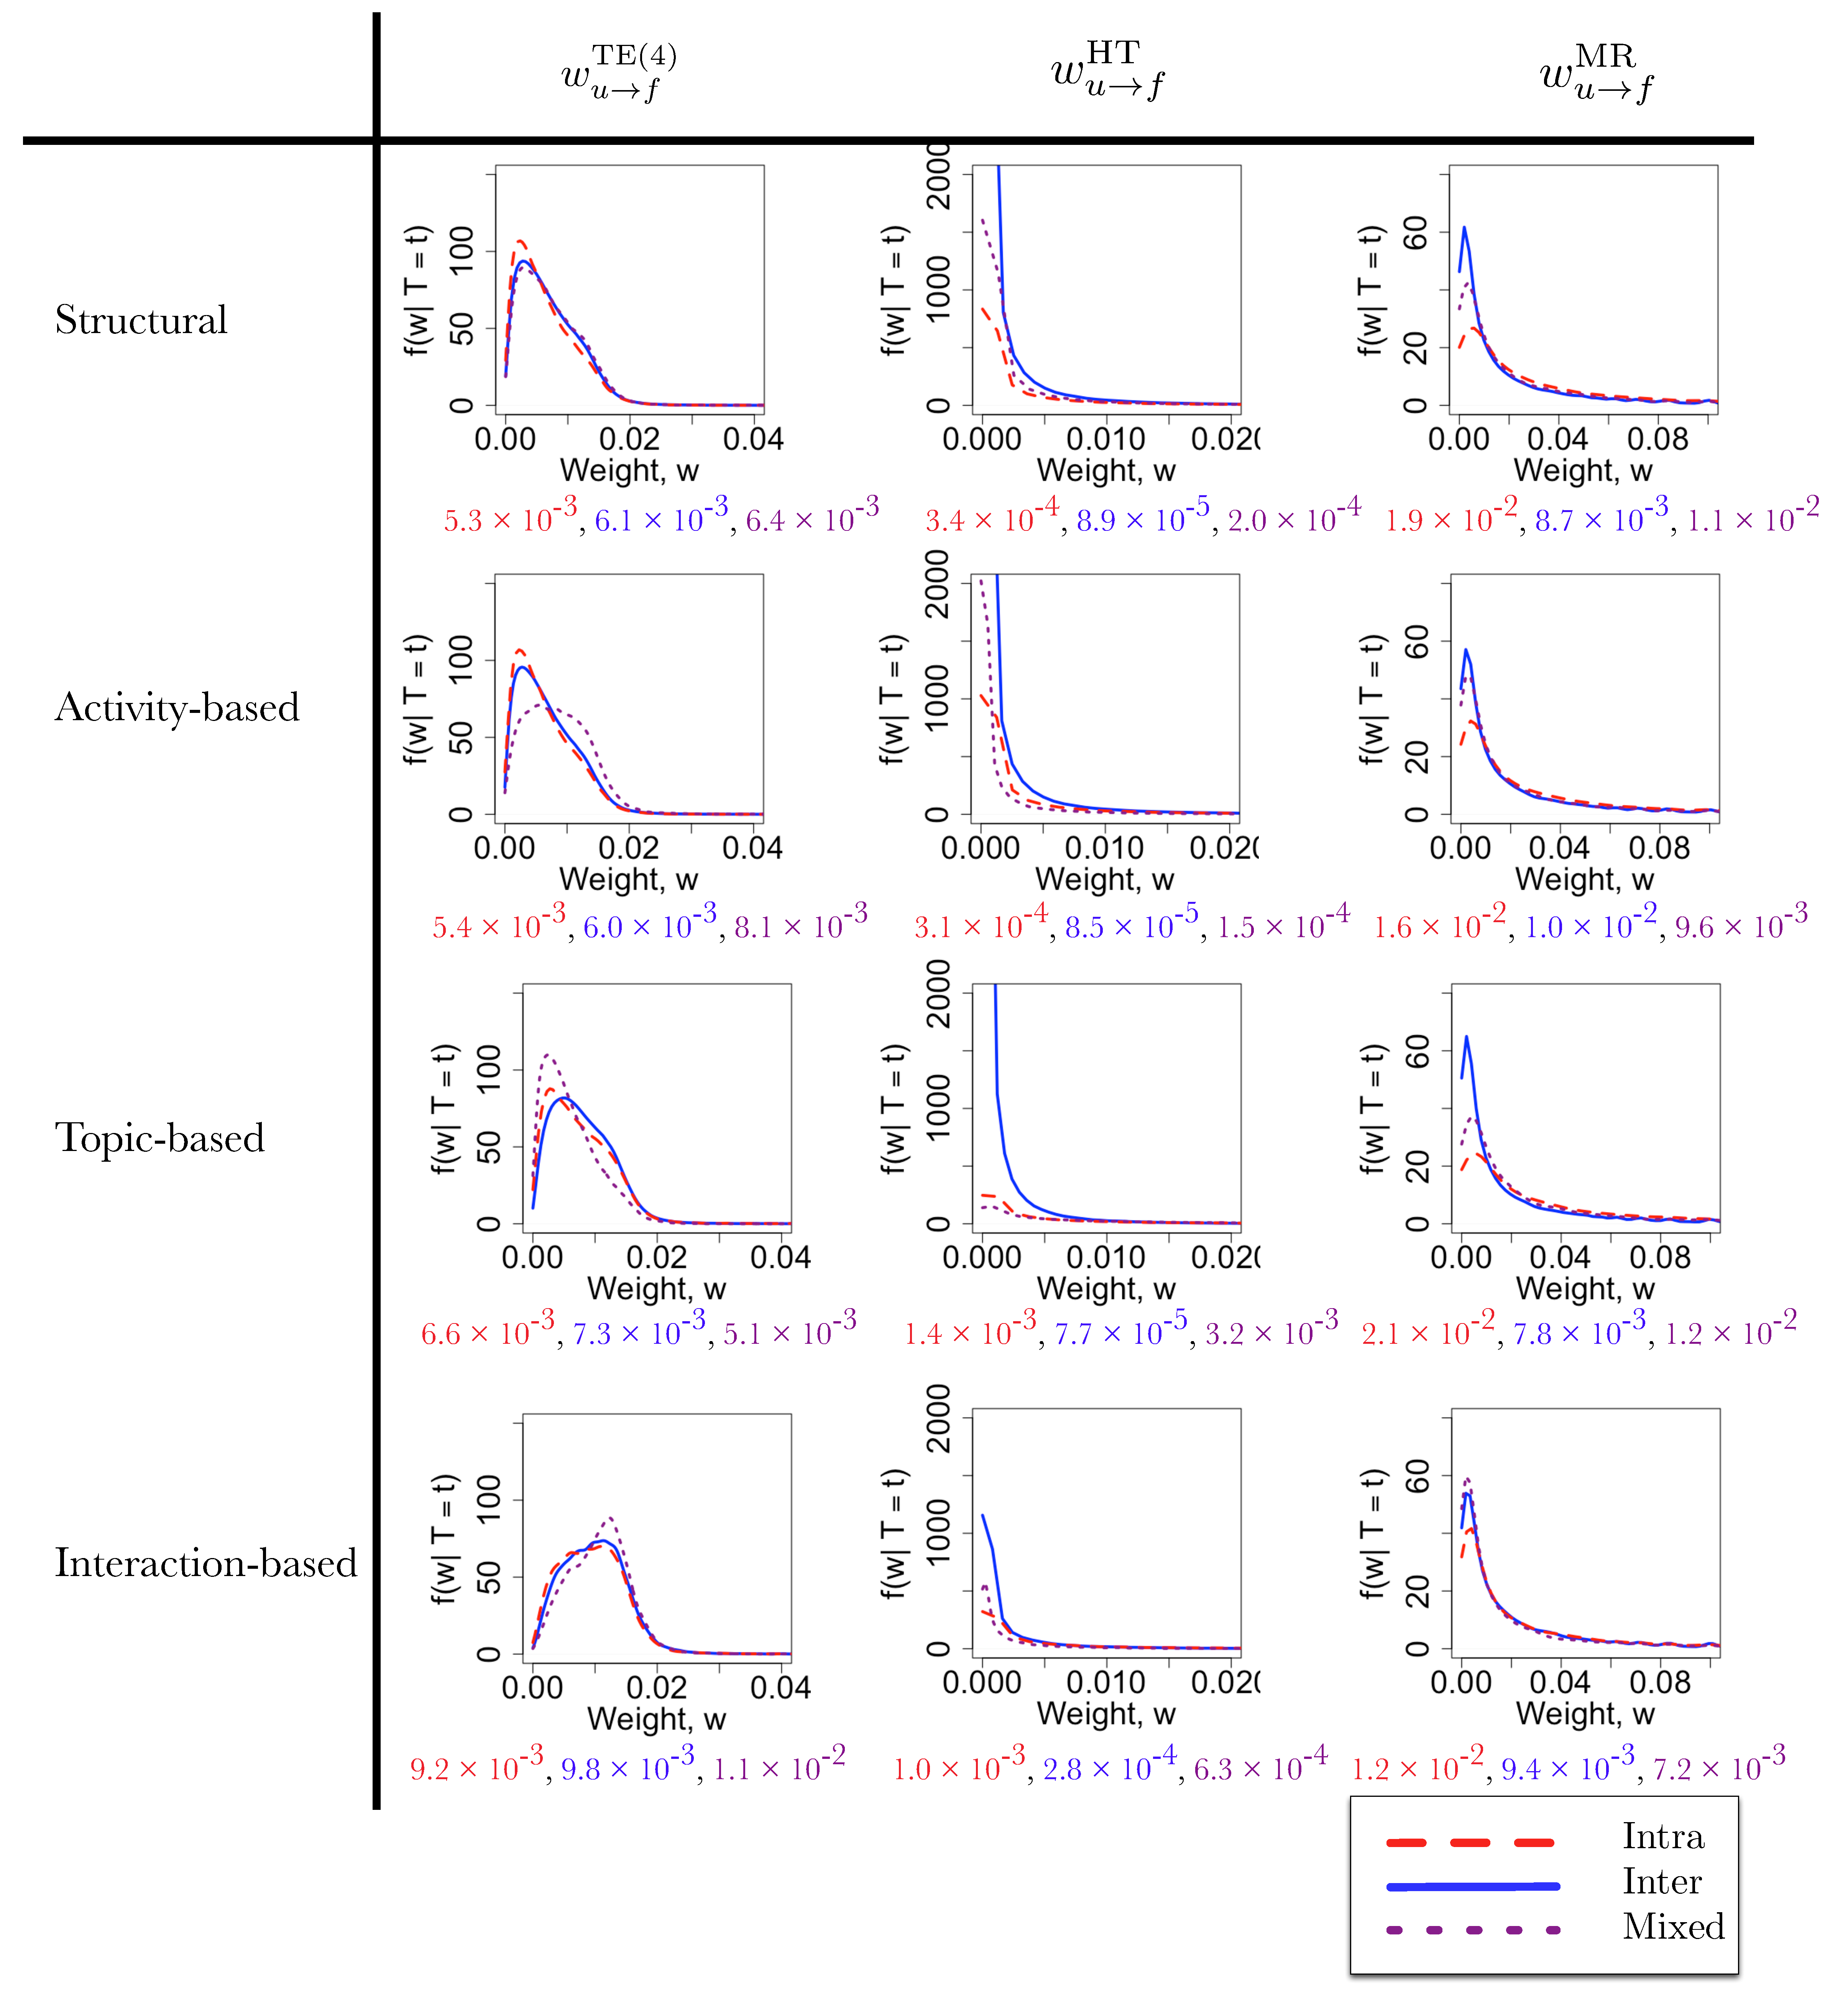
\includegraphics[width=1\textwidth]{densities-edges}
	\caption{The density of edge weights for different community types (rows) and weight types (columns). The red,  blue, and purple values below each collection of densities indicate the median of weight on intra-, inter-, and mixed-edges, respectively.}
	\label{Fig-distributions_by_types}
\end{figure}

Each \emph{column} of Figure~\ref{Fig-distributions_by_types} demonstrates how the density of weights change with the community type used to induce the partition. For example, the second column shows how the density of hashtag weights change based on the community partition. In general, the densities differ in non-trivial ways across the edge types and coverings. However, we see that the medians of the distributions provide a useful summary statistic. Under each collection of density functions, we list the median value of the inter, intra, and mixed-edges in red, blue, and purple, respectively. Unsurprisingly, we see that the greatest difference between the distributions occurs when we consider matching Community-type / Weight-type pairs, since the communities are determined based on the corresponding weights. However, we also see differences in the distributions when the Community-type / Weight-type pairs do not match. For example, for the covering corresponding to the activity-based communities, the hashtag weights tend to be higher for edges internal to communities than between communities. Similarly, for the covering corresponding to the topic-based communities, the transfer entropy weights tend to be higher on edges within (intra) and between (inter) communities, and lower for edges between members with multiple, non-identical memberships (mixed).

We also note that the distribution of transfer entropy weights always tend to be higher for edges crossing community boundaries (inter- or mixed-edges) compared to those edges within community boundaries (intra-edges). This is a property not exhibited by either the hashtag or mention-retweet weights, independent of the covering used to partition the edges. Moreover, for all but the activity-based covering, the weights of mixed-edges tend to be highest overall.  Recall that the transfer entropy $\text{TE}_{X(u) \to X(f)}$ quantifies the reduction in uncertainty about a follower $f$'s activity from knowing the activity of a user $u$. This result therefore implies that, in terms of prediction, it is more useful to know the time series of a user followed outside of the community compared to a user followed inside of the community, and even more useful to know the time series of a user that shares some, but not all, of the same community memberships. Thus, in an information theoretic sense, we see that novel information useful for prediction is more likely to flow \emph{across} community boundaries than \emph{within} community boundaries.

% \subsection{Demonstration of the Question-Oriented Approach}
%
% Next, we demonstrate a particular instance of a question-oriented approach. Suppose we were interested in tracking where conversations occur in a social network. That is, we want to track groups of individuals who interact more with each other than with users outside of their group. For example, we might wish to select a seed group of individuals in order to spread a message to a subpopulation of a social network. We now demonstrate how the performance on this tracking problem depends on the community type under consideration.
%
% % * We want to track *where* conversations are occurring: amongst what group of people.
%
% % * This motivates using the interaction-based communities.
%
% The data set was divided into two disjoint time periods: from 9am April 25th 2011 to 9am May 23rd 2011 (28 days) and from 9am May 23rd 2011 to 9am June 25th 2011 (33 days). We then constructed the three weighted networks (the structural network is unchanged) using the activity, retweets, mentions, and hashtags from the first time period, as described in the methodology section. Using the coverings inferred by OSLOM for the weighted network, we define the inside and outside of a community in the same way as depicted in Figure~\ref{Fig-edge_types}, where now we consider mixed-type edges to be internal. Based on this partitioning of the edges, we then track how many of the retweets / mentions in the second time period fall inside vs outside of the communities. The percentages of retweets and mentions that occur internal to each of the community types are given in Table~\ref{Tab-mentionretweets}.
%
% \begin{table}
% 	\caption{The percentage of retweets and mentions that occur internal to communities for each of the four community types.}
% 	\centering
% 	\begin{tabular}{l | c c}
% 		Community Type & Percentage of Retweets Internal & Percentage of Mentions Internal \\
% 		\hline
% 		Structural & 47.5 & 70.9 \\
% 		Activity-based & 54.7 & 75.6 \\
% 		Topic-based & 49.4 & 66.8  \\
% 		Interaction-based & \textbf{67.2} & \textbf{84.2}
% 	\end{tabular}
% 	\label{Tab-mentionretweets}
% \end{table}
%
% Let $I_{c}$ be the number of conversations (defined as a retweet or mention) occuring internal to community $c$, and let $|\mathcal{C}|_{c}$ be the size of community $c$. Finally, let $N$ be the total number of conversations, both internal and external, involving the nodes. An alternative scoring function is then
% \begin{align}
% 	\frac{1}{N}\sum_{c} \frac{I_{c}}{|\mathcal{C}_{c}|}.
% 	\label{conversation-metric}
% \end{align}
% That is, this measures the average number of internal conversations per user in a community. This will be maximized when the communities are small and the number of internal conversations are large compared to the total number of conversations.
%
% \begin{table}
% 	\caption{The metric (\ref{conversation-metric}) for the four community types, computed using the held-out data.}
% 	\centering
% 	\begin{tabular}{l | c c}
% 		Community Type & Retweets & Mentions \\
% 		\hline
% 		Structural & 0.0289 & 0.0344 \\
% 		Activity-based & 0.0793 & 0.0645 \\
% 		Topic-based & 0.1031 & 0.1020  \\
% 		Interaction-based & 0.0690 & 0.0977
% 	\end{tabular}
% 	\label{Tab-mentionretweets2}
% \end{table}
%
% \begin{table}
% 	\caption{The value of the conversation metric proposed by Elisa, averaged over all of the communities in a given covering.}
% 	\centering
% 	\begin{tabular}{ l | c c}
% 		Community Type & Mentions & Retweets \\
% 		\hline
% 		Structural & 2.9347 & 0.4734 \\
% 		Activity-based & \textbf{3.3893} & 0.5173 \\
% 		Topic-based & 2.5944 & 0.5580 \\
% 		Interaction-based & 2.1984 & \textbf{1.1069}
% 	\end{tabular}
% \end{table}

%\subsection{Qualitative Analysis of Community Memberships Across Types}
%\subsection{Answering the Questions}
\subsection{Uncovering the Multifacetedness of Community Memberships}

%As demonstrated by~\cite{good2010performance} in the context of modularity maximization-based community detection, an exponential number of nearby partitions may exist that nearly maximize an objective function used to measure the goodness-of-fit of a graph partition used for community detection. Because of this and related issues, it is always wise to perform some sort of qualitative study of the communities returned by any  community detection algorithm to verify their meaningfulness with respect to the scientific question at hand. In this section, we consider a collection of communities in such a study.

In the previous sections we showed that the communities emerging from the different weightings of the structural network quantitatively differ both at the macroscopic and at the microscopic scale. Here, we present some concrete examples of different community membership, in order to provide a practical illustration of the utility of using a multifaceted approach to community detection. We explore this first on a community level and then at the individual level.

In the topic-based communities, we found a single community consisting of 83 users who tweet about environmental issues and frequently use hashtags such as \#green, \#eco and \#sustainability. We also found a different community of 47 users who tweet about small businesses and entrepreneurship, using hashtags such as \#smallbiz, \#marketing and \#enterpreneur. In both cases, almost all members of these topic-based communities are not found in the same community in the other networks \emph{e.g.,} interaction- or activity-based, indicating that while these people talk about the same things and can therefore be considered a community based on their content, they do not strongly interact with each other nor behave the same, and so belong to different social groups with respect to interactions and behavior. This illustrates that the topics discussed by these users only define one facet of the users complex social network. 

Another interesting example is a community whose topics tend to focus on Denver and Colorado. These users do not belong to the same community in the interaction-based network, but most of them do belong to the same community in the activity-based network. This indicates that these users react to the same events and issues regarding Colorado and are therefore strongly connected in the topic-based and activity-based networks, but at the same time they do not directly interact with each other and are therefore more loosely connected in the interaction-based networks, where they belong to different communities.

It is interesting to examine the intersection between this topic-based community and the overlapping activity-based communities and explore which users in the intersection of these community types have the highest APC. Users with the highest APC in an activity-based community would provide the highest reduction in uncertainty on average about that communities activity or inactivity on Twitter. Interestingly, among the highest APC users in these communities---those with highest transfer entropy on average---we find $@$Colorado, which is the state official Twitter account, $@$ConnectColorado, a page created to connect Coloradans, and the CBS Denver account, a popular news agency. This means that these accounts have high activity-based predictive capacity in terms of their followers' activity on Twitter. This is not surprising as these activity-based communities heavily overlapped with the topic-based communities that discuss Colorado (mentioned above) and these accounts provide information on this topic. This provides a brief proof of concept that the APC measure makes sense and suggests this could be a useful measure for identifying individuals who possess high activity-based predictive capacity for a communities activity on a social media network. However, more work needs to be done to quantify this more fully.

At the individual-based level, we also found interesting examples of multifaceted community membership, which show that asking multiple questions leads to finding different kinds of communities a user belongs to. For example, the user $@$JohnReaves belongs to two different topic communities: one about health care and the other about `innovation' and `creativity'. There was a $~70\%$ overlap between the innovation and creativity topic community, the interaction-based, and the activity-based community the user is in, whereas there is almost no overlap between the latter two and the healthcare community. This means that the user interacts with and behaves like the people talking about innovation and creativity, but even though he also talks about healthcare he does not interact with (nor behave like) the people talking about that.
Another interesting example is given by user $@$jenajean. She  belongs to two different topic communities: she talks about NASA and space but she does not interact nor behave like people belonging to that topic community, whereas she also talks about leadership, and the people she interacts with highly overlap with the people belonging to the topic-based community on leadership for which she belongs to.
Lastly, $@$rajean, $@$Tekee, $@$Kimbirly and $@$mamamonroe are examples of users belonging to the topic community talking about Denver and Colorado. The activity-based community they belong to highly overlaps with the topic community (therefore they behave like the people that talk about Colorado), but they all belong to different interaction-based communities, each of which does not overlap in more than two users with the topic community.

\section{Discussion}
\section{Conclusion and Future Work}

\DIFaddbegin \label{sec:conc}

\DIFaddend % What have we done:
% ==================

%In this study, we have demonstrated that the communities observed in online social %networks are highly question-dependent 
%[[Joshua:maybe reword this sentence to explicitly say what we mean by question-dependent", might be a little confusing]]
%, and that different definitions of communities reveal different relationships between users. More importantly, we have shown that these different views of the network are not revealed by using the structural network alone. We found that community structure differs across community types on both the macro (e.g. number of communities and their size distribution) and micro (e.g. specific memberships, comemberships) scale.

In this study, we have demonstrated that the communities observed in online social networks are highly question-dependent. The questions posed about a network \emph{a priori} have a strong impact on the communities observed.  Moreover, using different definitions of community reveal different and interesting relationships between users. More importantly, we have shown that these different views of the network are not revealed by using the structural network or any one weighting scheme alone. By varying the questions we asked about the network and then deriving weighting schema to answer each question, we found that community structure differed across community types on both the macro ({\it e.g.,} number of communities and their size distribution) and micro ({\it e.g.,} specific memberships, comemberships) scale in interesting ways.

%We have also demonstrated that boundaries between communities represent meaningful internal/external divisions, with conversations and topics tending to be most highly concentrated within communities than without. We found this to be the case even when the communities were defined by a different criteria from the edge weights. [[Wasn't this the opposite in the transfer entropy case? Maybe I am remembering wrong. If so maybe we can spend a few sentences explaining why this is so leading into the next paragraph]]

To verify the validity of these communities we demonstrated that boundaries between communities represent meaningful internal/external divisions. In particular, conversations ({\it e.g.,} retweets and mentions) and topics ({\it e.g.,} hashtags) tended to be most highly concentrated within communities. We found this to be the case even when the communities were defined by a different criterion from the edge weights under study. 

% At first glance the boundaries defined by the communities in the activity-based network (those weighted with transfer entropy) seemed less meaningful. However, upon further investigation our novel use of transfer entropy for the detection of activity-based communities\footnote{It should be noted that while in previous work on online social media~\cite{ver2012information}, transfer entropy was found useful for identifying influence between users, it has not to the best of our knowledge been used to aid in the identification of communities.} brought to light a very interesting fact about this social network: influence tends to be higher across community boundaries than within them. This result echos the `strength of weak ties' theory from~\cite{granovetter1973strength}, which was supported empirically in~\cite{grabowicz2012social}. This means that our novel use of transfer entropy not only defines boundaries that are meaningful divisions between communities but it helps illustrate that influential users of a community need not be a member of that community.  

% Removed the footnote.

At first glance the boundaries defined by the activity-based communities derived from the transfer entropy weighting seemed less meaningful. However, upon further investigation our novel use of transfer entropy for the detection of activity-based communities highlighted an important fact about this social network: \DIFdelbegin \DIFdel{influence }\DIFdelend \DIFaddbegin \DIFadd{information transmission }\DIFaddend tended to be higher across community boundaries than within them. This result echos the `strength of weak ties' theory from~\cite{granovetter1973strength}, which has found empirical support in online social networks~\cite{grabowicz2012social}. This means that our use of transfer entropy not only defines boundaries that are meaningful divisions between communities but also illustrates that users who have a strong \DIFdelbegin \DIFdel{influence }\DIFdelend \DIFaddbegin \DIFadd{PV-AC }\DIFaddend on a community need not be a member of that community. 


%Start of future work**
Our findings may have important implications to a common problem in social network analysis: identification of influential individuals---but further work must be carried out.
\DIFaddbegin 

\DIFaddend Many network measures of influence are based on the various types of centrality (degree, betweenness, closeness, eigenvector, etc.)~\cite{newman2009networks}. Most centralities depend explicitly on the structure of the network under consideration. But we have seen in our study that \DIFdelbegin \DIFdel{a structural network alone is not sufficient to capture user interaction or even activity-based influence in }\DIFdelend \DIFaddbegin \DIFadd{the structural network only highlights one of many possible ways that users interact with }\DIFaddend online social media.
Thus, a na\"ive application of centrality measures to a structural network \DIFdelbegin \DIFdel{for influence detectionmay give rise to erroneous results. This result }\DIFdelend \DIFaddbegin \DIFadd{may be answering a different question than the one motivating influence detection. For example, a user exhibiting high closeness centrality based on the structural network may be able to make a message visible to most other users in a social network, but this does not mean that those other users are likely to respond to or propagate that message. The importance of correctly framing network measures of influence }\DIFaddend has been explored previously~\cite{kitsak2010identification}, and our work further highlights its importance. 

Based on our preliminary results, we conjecture that weighted generalizations of these centrality measures using transfer entropy might lead to better insights about who is actually influential in an online social network. 
\DIFaddbegin \DIFadd{It is interesting to note for example that two of the Forbes ``Top 10 Social Media Influencers", happen to be in our network, }\emph{\DIFadd{viz.}}\DIFadd{, Ann Tran and Jessica Northey, and transfer entropy also quantified these two users as having high PV-AC, i.e., the uncertainty about their followers activity on Twitter was reduced given their tweet histories. While we do not believe this information theoretic measure can capture social influence in its entirety, 
%DIF >  members, as categorized by transfer entropy. 
this suggests that this activity-based measure may be useful in finding influential members purely based on their temporal tweet history; even completely ignoring both tweet content and social status. However, a deeper analysis would need to be carried out to verify this finding.
}\DIFaddend In addition to exploring this phenomenon further, we plan to explore a broader selection of choices for both the transfer-entropy lag and tweet history time resolution. We believe that by doing an in-depth analysis of both of these parameters we can discover interesting activity-based communities that occur on much broader time scales.
%End of futre work**
  %based on methods for model selection~\cite{claeskens2008model}.

%Our work has introduced a novel use of transfer entropy for the detection of activity-based communities. 


%Our transfer entropy results thus reflect that influence tends to be higher across community boundaries than within them. This result echos the `strength of weak ties' theory from~\cite{granovetter1973strength}, which has found empirical support in~\cite{grabowicz2012social}. In addition to exploring this phenomenon further, we plan to consider more rigorous choices of both the lag and time resolution based on methods for model selection~\cite{claeskens2008model}.




% * Defined four types of communities based natural questions one might ask about users in online social media.

% * Proposed three weightings to detect such communities.

% * Demonstrated that the community structure differed between weighting to weighting.

% Future Work:
% ============

% More with transfer entropy.
% 	Why did information tend to flow *across*, rather than within, community boundaries?

% Longitudinal study:
% 	How do the different types of communities change over time? Are activity-based communities more stable than interaction-based, etc.? For example, preliminary studies indicate that `conversations,' as defined by mentions and retweets, tend to move outside of structural communities over time.

%[[This paragraph needs to be recrafted a bit. It just reads a little confusing]]

%Our work has introduced a novel use of transfer entropy for the detection of activity-based communities. In previous work on online social media~\cite{ver2012information}, transfer entropy was found useful for identifying influence between users. Our transfer entropy results thus reflect that influence tends to be higher across community boundaries than within them. This result echos the `strength of weak ties' theory from~\cite{granovetter1973strength}, which has found empirical support in~\cite{grabowicz2012social}. In addition to exploring this phenomenon further, we plan to consider more rigorous choices of both the lag and time resolution based on methods for model selection~\cite{claeskens2008model}.

% Why Care? (i.e. impact):
% ========================

% What does this mean for researchers in online social media? Businesses?

% Using concepts like centrality to determine influence 
% 	* These metrics are based solely on the structural network.
% 	* Your *activity* may be more important than your *topology* in determining
% 	  your influence.
%[[While I agree with this next paragraph completely I am not sure we covered this topic enough to be the final paragraph of the conclussion or even in the conclusion. I need to think about this...]]

% More generally, our work demonstrates that asking the proper question is an unavoidable first step to community detection, and that the rich data sets available from 

This work demonstrates \DIFdelbegin \DIFdel{that asking the proper question, and then crafting an appropriate weighting scheme to answer that question}\DIFdelend \DIFaddbegin \DIFadd{the utility of a multifaceted question-oriented approach to community detection. This work shows that crafting }\emph{\DIFadd{several}} \DIFadd{facet-driven weighting schema, doing community detection for each weighting scheme and then comparing the similarities and differences across community types}\DIFaddend , is an unavoidable \DIFdelbegin \DIFdel{first step for community detection }\DIFdelend \DIFaddbegin \DIFadd{process for uncovering the hidden layered community structure present }\DIFaddend in online social \DIFdelbegin \DIFdel{media}\DIFdelend \DIFaddbegin \DIFadd{networks}\DIFaddend . More generally, this work illustrates that without a clear definition of \DIFdelbegin \DIFdel{community, many }\DIFdelend \DIFaddbegin \DIFadd{community---or even only using a }\emph{\DIFadd{single}} \DIFadd{definition of community---many }\DIFaddend rich and interesting communities present in online social networks remain invisible. \DIFdelbegin \DIFdel{Question-oriented }\DIFdelend \DIFaddbegin \DIFadd{Multifaceted question-oriented }\DIFaddend community detection can bring those hidden communities into the light.



\bibliography{references}
\bibliographystyle{aaai}

\end{document}